\documentclass[headsepline]{scrreprt}

%\usepackage{isolatin1}
%\usepackage[latin1]{inputenc}
\usepackage{amsfonts,amsthm} %% used for mathbb -> R
%\usepackage{euscript}
\usepackage{url,booktabs}
\usepackage{graphicx}
%\usepackage{algorithm,algorithmic}
\usepackage{textcomp}  % for
%\usepackage[activate=normal]{pdfcprot}
\usepackage[bf,small]{caption2}  %% Bessere Bildunterschriften
\usepackage{color,longtable}
\usepackage{subfigure}
\usepackage{tabularx}
\usepackage{listings}
\usepackage{amsmath}
\usepackage{amssymb}
\usepackage{booktabs}
\usepackage{fancybox}
\usepackage{pifont}
\usepackage[round,comma]{natbib}
\usepackage{hyperref}
\usepackage{moreverb,listings,MnSymbol}

%%% Kommandos... fuer Bildpositionierung?
\renewcommand{\textfraction}{0.15}
\renewcommand{\topfraction}{0.85}
\renewcommand{\bottomfraction}{0.65}
\renewcommand{\floatpagefraction}{0.60}
\newcommand{\dotl}{\stackrel{.}{<}}
\newcommand{\dotg}{\stackrel{.}{>}}
\definecolor{grau}{gray}{0.5}

\newcommand{\secref}[1]{Section #1}
\newcommand{\figref}[1]{Figure #1}

\theoremstyle{definition}
  \newtheorem{defn}{Definition}
  \newtheorem{lemma}{Lemma}
  \newtheorem{theo}{Theorem}
  \newtheorem{koro}{Corollary}

%\setkomafont{section}{\rmfamily}
%\setkomafont{chapter}{\rmfamily\huge}
%\setkomafont{subsection}{\rmfamily}
%\setkomafont{subsubsection}{\rmfamily}
%\setkomafont{paragraph}{\rmfamily}


%\usepackage{acronym}

% F\"ur andere Haken siehe Seite 7 in http://www.tug.org/tex-archive/macros/latex/required/psnfss/psnfss2e.pdf
\newcommand{\haken}{\ding{51}}
\newlength{\platz}
\newlength{\einrueck}
\settowidth{\einrueck}{\bfseries{\sffamily{calculus parameters: }}}
\newlength{\rest}
\newlength{\kastenbreite}
\setlength{\kastenbreite}{130mm}
\setlength{\rest}{\kastenbreite}\addtolength{\rest}{-1\einrueck}
\addtolength{\rest}{-1mm} % Der rechte Rand beim Kasten ist mir zu klein...
\newenvironment{calcfeatures}{\begin{tabbing}\hspace*{\einrueck}\= \\[-1ex]}{\vspace*{-1cm}$ $\end{tabbing}}
\newcommand{\feature}[2]{{\bfseries{\sffamily{#1}}}\>\parbox[t]{\rest}{\sf #2}\\[1.5ex]}
\newcommand{\lastfeature}[2]{{\bfseries{\sffamily{#1}}}\>\parbox[t]{\rest}{\sf #2}}

\newlength{\shellbreite}
\setlength{\shellbreite}{\textwidth}
\addtolength{\shellbreite}{-5mm}
\definecolor{hellgrau}{gray}{0.85}
\newcommand{\shellThree}[3]{\medskip\noindent\centerline{\colorbox{hellgrau}{\parbox{\shellbreite}{\medskip\small \tt \$ #1\\ "#2"\\ > #3\medskip}}}\medskip}
\newcommand{\shell}[2]{\medskip\noindent\centerline{\colorbox{hellgrau}{\parbox{\shellbreite}{\medskip\small \tt \$ #1\\ > #2\medskip}}}\medskip}
\newcommand{\cmdline}[1]{\medskip\noindent\centerline{\colorbox{hellgrau}{\parbox{\shellbreite}{\medskip\small \tt \$ #1\medskip}}}\medskip}
\newcommand{\outp}[1]{\medskip\noindent\centerline{\colorbox{hellgrau}{\parbox{\shellbreite}{\medskip\small \tt #1\medskip}}}\medskip}


\newcommand{\ul}{\hspace*{-0.1em}\rule{0.65em}{1pt}}
\newsavebox{\notetext}
\savebox{\notetext}{\bfseries{Note: }}
\newlength{\platznote}
\settowidth{\platznote}{\usebox{\notetext}}
\setlength{\platznote}{-1\platznote}
\addtolength{\platznote}{\textwidth}
\newcommand{\note}[1]{\noindent\usebox{\notetext}\parbox[t]{\platznote}{#1}}

\newcommand{\binaryonly}{\raisebox{1ex}{\scriptsize(2)}}
\newcommand{\ternaryonly}{\raisebox{1ex}{\scriptsize(3)}}

%\medskip {\bf Note:} \parbox{\fill}{#1}}

\graphicspath{{figures/}}

\newcommand{\R}{\mathbb{R}}
\newcommand{\argmax}{\mathop{\mathrm{argmax}}}
\newcommand{\argmin}{\mathop{\mathrm{argmin}}}

\newcommand{\sfbsc}{SFB/TR\,8 Spatial Cognition}
\newcommand{\qshape}{R3-[Q-Shape]}
\newcommand{\engine}{SparQ}
\newcommand{\opra}{$\mathcal{OPRA}_m$}
\newcommand{\OPRAm}{$\mathcal{OPRA}_m$}
\newcommand{\opraeins}{$\mathcal{OPRA}_1$}
\newcommand{\oprazwei}{$\mathcal{OPRA}_2$}
\newcommand{\opradrei}{$\mathcal{OPRA}_3$}

\newcommand{\DRAc}{$\mathcal{DRA}_{c}$}
\newcommand{\DRAf}{$\mathcal{DRA}_{f}$}
\newcommand{\DRAfp}{$\mathcal{DRA}_{fp}$}
\def\LR{$\mathcal{LR}$}


% \newcommand{\kasten}[1]{\begin{minipage}{.5\linewidth}
% \setlength{\fboxrule}{0.3mm} \hspace{0.5cm}
% \fcolorbox{black}{yellow}{\parbox{120mm}{\small #1}}
% \end{minipage}}

\newcommand{\kasten}[1]{\begin{minipage}
{.5\linewidth}
\setlength{\fboxrule}{0.4mm} \hspace{0.5cm}
\shadowbox{\parbox{\kastenbreite}{{\small #1}}}
\vspace{1mm}
\end{minipage}}
\def\shadowsize{2.5pt}

%\newcommand{\kastenwidth}{11.8cm}

\newcommand{\uline}{\rule[-0.2ex]{0.5em}{1pt}}

%
% remark
%
% uncomment this line to show remarks
%\newcommand{\remark}[1]{\marginpar{#1}}
% uncomment this line to hide remarks
\newcommand{\remark}[1]{}


\pagestyle{headings}



%\lstset{language=LISP,basicstyle=\footnotesize\tt,stepnumber=5,
%  numbers=left,numberstyle=\tiny,showstringspaces=false,float=htp,captionpos=b,
%  emptylines=0
%}
\lstset{ %
language=Lisp,
numbers=none,
basicstyle=\footnotesize\tt,
showstringspaces=false,
breaklines=true,
breakatwhitespace=true,
morekeywords={:requires,:documentation,def-tool},
prebreak=\mbox{{\color{blue}$\lcurvearrowse$}},
postbreak=\mbox{{\color{blue}$\dashrightarrow$}},
frame=single
}


%\subject{\sfbsc\ - Project \qshape}
\title{\engine\ User Manual V0.8}
\author{Diedrich Wolter\\ Jan Oliver Wallgr{\"u}n \\ Frank Dylla\\ Lutz Frommberger}
\date{\today}


\newcommand{\changefont}[3]{
\fontfamily{#1} \fontseries{#2} \fontshape{#3} \selectfont}

\setkomafont{sectioning}{\changefont{cm}{bx}{n}}


\begin{document}

%\begin{center}\framebox{\parbox{15cm}{Noch zu tun:\begin{itemize}
%        \item Implementation details (4.1)
%	\item Algebraische Spezifikiation und Quantifizierung beschreiben
%\end{itemize}}}\end{center}

\begin{titlepage}
\begin{center}
{\huge \bfseries{\engine\ User Manual V0.8\\}}
\bigskip
{\LARGE September 2014\\ \bigskip
Diedrich Wolter\\ Jan Oliver Wallgr{\"u}n \\ Frank Dylla\\ Lutz Frommberger\\
}
\end{center}
\vfill
\begin{tabular}{llll}
\multicolumn{2}{l}{Further contributions by:}\\[1ex]
Dominik L\"ucke & Thomas Schneider &  & \\
\end{tabular}
\vfill
\end{titlepage}
%\maketitle
\tableofcontents


\chapter*{About SparQ...}


\engine{} is a toolbox for representing space and reasoning about
space based on  qualitative spatial relations. Its development started
within the \qshape{} project of the Spatial Cognition Research Center in Bremen, Germany in 2006.
Financial support by the the Deutsche Forschungsgemeinschaft (DFG)  is gratefully acknowledge.
By now, contributors have moved on and so has \engine{}.

\engine{} disseminates results from the qualitative spatial and temporal reasoning community which consists of researchers from a various disciplines
including computer science, artificial intelligence, geography, philosophy,
psychology, and linguistics.
So far, a multitude of formal calculi over sets of
spatial relations (like `overlaps', `left-of',
`north-of') have been proposed, focusing on different
aspects of space (mereotopology, orientation, distance, etc.) and
dealing with different kinds of objects (points, line segments,
extended objects, etc.). \engine{} aims at making these qualitative spatial
calculi and the developed reasoning techniques available in a single
homogeneous framework that is released under the GPL license for freely available software and can easily be included into applications.
Our aim is providing a common toolbox spanning across all techniques of qualitative reasoning, thereby providing a universal toolbox to the user. Currently, we provide techniques for
\begin{itemize}
	\item specifying qualitative formalisms and analyzing them
	\item interfacing the continuos domain with qualitative representations
	\item manipulating symbolical propositions
	\item reasoning with symbolical propositions, in particular checking consistency of qualitative information
	\item interfacing with other reasoning tools
\end{itemize}

\engine{} is designed for the application designer or researcher working in a field other than qualitative reasoning, offering access to reasoning techniques in an easy-to-use manner. If you  are new to qualitative spatial reasoning, see the following chapter for an introduction to this field and the services it can offer to your field.

SparQ is also designed for the researcher working on qualitative spatial and temporal reasoning (QSR). It provides an implementation toolbox of key techniques in QSR, making experimental analysis easier. Furthermore, SparQ offers an easy format to specify new calculi. This eases distribution of new calculi and enables researches to more easily compare different calculi, for example in an application context. In this manner SparQ is a community effort: it provides a rich repertoire of qualitative calculi to application designers. We would be happy to include your calculus! Last but not least, SparQ offers tools for analyzing QSR calculi, thereby supporting the calculus designer.


This document provides answers to four topic areas:
\begin{itemize}
	\item installation of SparQ
	\item brief introduction to the field of QSR
	\item reference of SparQ commands and calculi specification syntax
% (TBD!)	\item Detailed implementation notes and an outlook on planned extensions 
	\item brief description of provided calculi 
\end{itemize}

%Section \ref{sec:qsr} offers a small introduction to qualitative spatial calculi and qualitative spatial reasoning in general and introduces the relevant terms required for working with \engine{}.
%The spatial calculi currently supported by \engine{} are documented in Section \ref{sec:supp-spat-calc} of this manual. \engine{} is designed in a way that
%makes it easy to specify and integrate new calculi.


%For an up-to-date list of
%supported calculi and the newest version of this manual, please visit our
%website (\url{http://www.sfbtr8.uni-bremen.de/project/r3/sparq/}).
%Up to now, we focus on calculi for reasoning about the positions of points or line segments, but we hope to include more calculi in the future.
For questions or feedback, please get in contact with us an e-mail to the address below. We are always interested in suggestions for improvement and in hearing about your experience with \engine{}.

\vspace{0.5cm}
\noindent
The \engine{} team

\noindent
\url{qshape@sfbtr8.uni-bremen.de}

%\chapter{QSR---An Introduction} %(was ist die RI-Engine)
%\label{sec:introduction}

%The current version of \engine{} provides the following services (which will be thoroughly explained later in this manual):

%\begin{description}
%\item[qualification] --- A quantitative geometric description of a spatial configuration can be transformed into a qualitative description employing one of the supported spatial calculi.
%\item[computing with relations] --- The operations defined in a calculus (intersection, union, complement, converse, composition, etc.) can be employed to perform algebraic computations with the spatial relations from one of the supported calculi.
%%\item[computing with neighborhoods] computing with the conceptual neighborhood structures defined in for a calculus
%\item[constraint reasoning] --- Techniques for solving relational constraint satisfaction problems (CSPs) based on the supported calculi can be used to check the consistency of spatial information, determine if a particular relation can hold between certain objects, or derive a concrete possible scenario from under-specified information.
%\end{description}

\section*{License}

SparQ is free software: you can redistribute it and/or modify
it under the terms of the GNU General Public License as published by
the Free Software Foundation, either version 3 of the License, or
(at your option) any later version.

 This program is distributed in the hope that it will be useful,
 but WITHOUT ANY WARRANTY; without even the implied warranty of
 MERCHANTABILITY or FITNESS FOR A PARTICULAR PURPOSE.  See the
 GNU General Public License for more details.

A copy of the GNU General Public License is provided in the COPYING file
distributed with SparQ. If you can't access it, visit \url{http://www.gnu.org/licenses/}.

As this software is being provided free of charge,
warranty as stipulated in sections 11 and 12 shall be governed by the
provisions of German civil law concerning gifts (Schenkungsrecht).

\chapter{Installing \engine}
\label{sec:inst-ri-engine}

\engine{} is built using several standard tools available for a variety of operating systems. \engine{} is written for POSIX systems. Its functionality
is continuously tested on Linux, Solaris, and Mac OS X, but it should work on
any Unix system.


\section{Requirements}\label{sec:requirements}

\engine{} is currently not available in binary versions. For installation some freely available standard tools are required. Besides its calculi specifications as plain text, \engine{} comprises a set of C libraries and a main program written in Lisp. For compilation we rely on availability of these tools:
%It is available for
%POSIX systems (installation is explained in Section \ref{sec:inst-ri-engine}).
%The main program can either be used directly from the console or included into own applications via TCP/IP streams\footnote{Using the libraries directly is neither documented nor recommended as their interfaces have not been unified so far and not all parts of the toolbox come in the form of libraries.}. The details of using \engine{} are explained in Section \ref{sec:using-ri-engine}.

\begin{itemize}
	\item Steel Bank Common Lisp
          (SBCL)\footnote{\url{http://sbcl.sourceforge.net/}}, version~0.9.10 or higher
	\item gcc and g++, version 2.95 or higher
    \item GNU libtool, version 1.4.3 or higher\footnote{On Mac\,OS\,X a
            newer libtool version may be required, otherwise a manual patch may be
            necessary. See INSTALL notes for details.}
	\item \LaTeX{} for typesetting this manual
\end{itemize}

%The source code of the actual version of \engine{} and appropriate documentation is available at the
%\engine{}-homepage (\url{http://www.sfbtr8.uni-bremen.de/project/r3/sparq/}).

\section{Building the Executable}
To build a running version of \engine{}, unpack the source code package, enter
the newly created SparQ directory (called \verb|sparq-<version>|) and run
\label{sec:building-binaries}

\cmdline{./configure}

followed by

\cmdline{make}

The executable will be installed within the \engine{} directory. Please note that
you have to recompile \engine{} if you move the directory to another place.

If you encounter any problems during the build process, please contact the authors.



\chapter{Reasoning with Qualitative Spatial Relations}
\label{sec:qsr}

In this section, we provide a brief introduction on
qualitative spatial reasoning and explain the most
important terms required when dealing with qualitative
spatial calculi in \engine{}. For more in-depth introductions to
the field, we refer to \citet{cohn01_qsr_overview,cohn97_qsr_techniques,ladkin92_qualCSP,ladkin94_relalg,duentsch_05_relation},
and the references
provided for particular calculi in Appendix
\ref{sec:supp-spat-calc}.

\section{What is a Qualitative Spatial Calculus?}

A qualitative calculus consists of a set of relations between objects
from a certain domain and operations defined on these relations.
Let us start with an easy example: the spatial version of the Point Algebra (PA) \citep{vilain_kautz_beek_89_constraint}.
Imagine, we are being told about a boat race on a river by a friend on the
phone\footnote{This example has been borrowed from \citet{ligozat_05_categorical}.}.
We can model the river as an oriented line and the boats
of the 5 participants A,B,C,D,E as points moving along the line (see Fig.
\ref{fig:br0}). Thus,
our domain (the set of spatial objects considered) is the set of all
1D points.

\begin{figure}[ht]
	\centering
	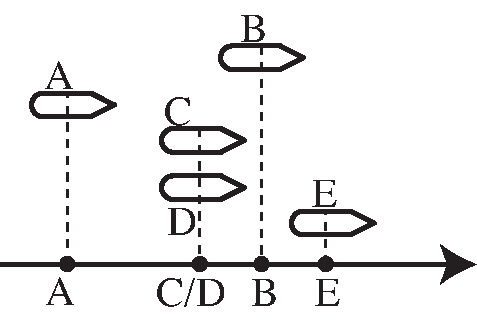
\includegraphics[width=0.5\textwidth]{boatrace_cn_0}
	\caption{A possible situation in a boat race which can be modeled by 1D points on an oriented line and be described by qualitative relations from the Point Algebra.}
	\label{fig:br0}
\end{figure}

We now distinguish three relations between objects from
our domain. A boat can be \emph{ahead} of another boat, \emph{behind} it,
or on the \emph{same} level. These relations can be used to formulate
knowledge about the current situation in the race. For instance, our
friend tells us the following:

\begin{enumerate}
\item A is \emph{behind} B
\item E is \emph{ahead} of B
\item A is \emph{behind} C
\item D is on the \emph{same} level as C
\item A is \emph{ahead} of D
\end{enumerate}
From this information we are able to conclude that our friend must have
made an error, probably confusing the names of the participants: We know
that A is \emph{behind} C (sentence~3) and D is \emph{behind} A (conversion of sentence~5). From
composing these two facts it follows that C and D cannot be on the \emph{same}
level which contradicts sentence 4.

On the other hand, only taking the first three sentences into account, we can conclude that E
is also \emph{ahead} of A by composing
the facts A is \emph{behind} B (sentence 1) and B is \emph{behind} E (conversion of sentence~2).
However, this information is not sufficient to derive the exact
relation
between C and E, as C can either be \emph{ahead}, \emph{behind} or on the {\em
same} level as E.

The calculus, in this case the PA, defines a set of base relations
(\emph{ahead}, \emph{behind}, and \emph{same}) and
provides the elementary reasoning steps in the form of operations defined
over the base relations. In our small example, the applied
operations were conversion, which given the operation between x and y returns
the relation between y and x (thus the converse of \emph{ahead} is
\emph{behind}), and composition which takes the relations holding
between X \& Y and Y \& Z and returns the relation holding between X \& Z (e.g.
composition of \emph{ahead} and \emph{ahead} is \emph{ahead}).

Often the result of operations like the composition operation is
not a single base relation but the union of more than one. For
instance, knowing that X is \emph{ahead} of Y and Y is \emph{behind}
Z yields the union of \emph{ahead}, \emph{behind}, and \emph{same}.
Because of this, the set of relations considered in a spatial
calculus is not just the set of base relations, but the set
of all unions of base relations including the empty set and
the union of all base relations (the universal relation).
All operations of the calculus are then defined for all unions
of base relations: For example, we can apply conversion to
the information that X is either \emph{ahead} or at the
\emph{same} level as Y to infer that Y is either \emph{behind}
or at the \emph{same} level as X.

\section{Constraint Networks, Consistency, and Consistent Scenarios}

A spatial configuration of a finite set of objects from the domain
as given by sentences 1--5 can be described as a \emph{constraint
network} as shown in Fig.~\ref{fig:br1}. It consists of a variable for each
object represented by the nodes of the network and edges
labeled with relations from the considered calculus denoted
as sets of base relations. For instance, sentence 1 is
represented by the edge going from A to B labeled with
$\{behind\}$. If no edge connects two nodes, this corresponds
to an edge labeled with the universal relation U (the union of all base relations expressing complete ignorance), which is
usually omitted.

\begin{figure}[ht]
	\centering
	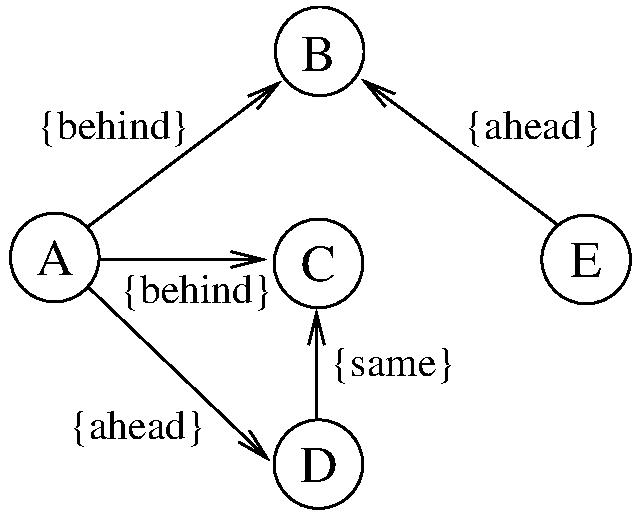
\includegraphics[width=0.4\textwidth]{boatrace_cn_1}
	\caption{The situation described by sentences 1--5 as a constraint network. }
	\label{fig:br1}
\end{figure}


As we have seen in our example, the information
given in a constraint network can be inconsistent. This means,
no objects from the domain can be assigned to the
variables so that all the constraints given by the spatial
relations annotated to the edges are satisfied. If,
on the other hand, such
an assignment can be found, the constraint network is
said to be \emph{consistent} or \emph{satisfiable} or \emph{realizable}.
Determining whether a constraint network is consistent is
a fundamental problem of qualitative spatial reasoning.
Special techniques for determining consistency based on the operations
of the calculus (especially the composition operations) have
been developed. However, it is important to note that
the soundness of these methods depends on the properties
of the calculus at hand and are often still subject of
ongoing investigations. For more details on this issue,
we refer to \citet{RenzL05_WeakComposition}
and the literature on individual
calculi listed in Appendix \ref{sec:supp-spat-calc}.

A constraint network in which every constraint between
two variables is a base relation is called \emph{atomic}
or a \emph{scenario}. This means all spatial relations
between two objects are completely determined with
respect to the employed calculus and the remaining
question is if the network is consistent or not.
However, if a constraint network contains relations
that are not base relations like in Fig.~\ref{fig:cn2},
we might also be interested in finding a scenario
that is a \emph{refinement} of the original network
(meaning it has been derived by removing individual base
relations from the sets annotated to the edges) and
that is consistent. Fig.~\ref{fig:cn3} shows such a
\emph{consistent scenario} for the network in
Fig.~\ref{fig:cn2}. If such a consistent scenario
can be found, we also know that the original network
is consistent. Otherwise, we know it is inconsistent.
Of course, it is possible that more than one
consistent scenario exists for a given constraint
network and we might be interested in finding
only one or all of these. An alternative
consistent scenario is depicted in Fig.~\ref{fig:cn4}.

\begin{figure}[ht]
	\centering
	\subfigure[]{
	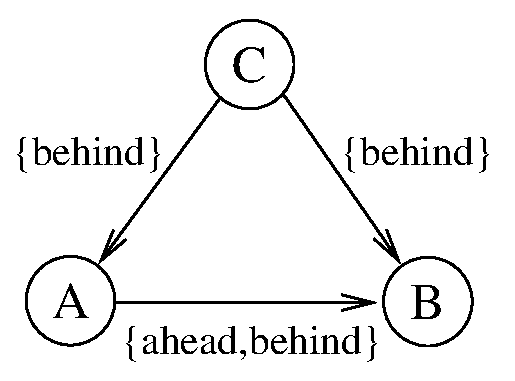
\includegraphics[width=0.28\textwidth]{boatrace_cn_2}
	\label{fig:cn2}
	}
	\subfigure[]{
	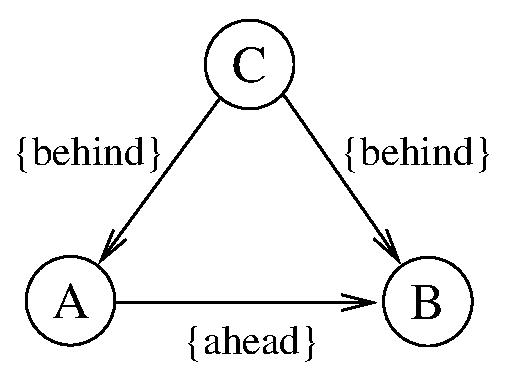
\includegraphics[width=0.28\textwidth]{boatrace_cn_3}
	\label{fig:cn3}
	}
	\subfigure[]{
	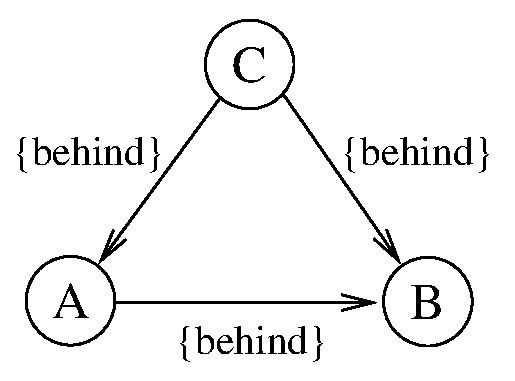
\includegraphics[width=0.28\textwidth]{boatrace_cn_4}
	\label{fig:cn4}
	}
	\caption{A non-atomic constraint network (a) with possible consistent
scenarios (b) and (c).}
	\label{fig:br2}
\end{figure}

The problems of determining consistency and finding consistent
scenarios are subsumed under the term
\emph{constraint-based reasoning} throughout this
text.

\section{Qualitative Constraint Calculi}

After giving a rather intuitive introduction to
qualitative spatial calculi, we want to give a more
formal definition of a spatial calculus and especially
the operations a calculus needs to define.

\begin{defn}[qualitative calculus, base relations, arity]
	A {\em qualitative calculus} $<\mathcal{B}, \mathcal{D}^n>$ defines a finite, non-empty set $\mathcal{B}$ of $n$-ary qualitative {\em base relations} over some domain $\mathcal{D}$, i.e. $\mathcal{B} \subseteq 2^{\mathcal{D}^n}$.
	We call $n$ the arity of the calculus.
\end{defn}

For the purpose of constraint reasoning one usually requires that the set of base relations
partitions $\mathcal{D}^n$.

\begin{defn}[JEPD]
	A qualitative calculus $<\mathcal{B}, \mathcal{D}^n>$ is called {\em jointly exhaustive}, if the base relations cover $\mathcal{D}^n$, i.e. $\bigcup_{B\in \mathcal{B}} B = \mathcal{D}^n$. The calculus is called {\em pairwise disjoint} if no two base relations overlap, i.e. $\forall B,B' \in \mathcal{B} \, :\, B \cap B' = \emptyset$. Jointly exhaustive and pairwise disjoint calculi are commonly referred to as JEPD calculi.
\end{defn}


In qualitative reasoning we consider a simple formal language that only allows relating (unqualified) objects by qualitative relations. Here, a infix notation is commonly used. For example, $A\, r\, B$ stands for $(A,B) \in r$. Uncertainty can be modeled by using
unions of base relations, e.g., to express that some objects may either stand in some relation $r$ or $s$ can be expressed by the relation $r \cup s$, usually denoted $\{r,s\}$\footnote{The notation using sets like $\{r,s\}$ can be misleading as it syntactically identifies sets of relations with their unions. However, this notation is the established form.}.

\begin{defn}[general relations]
	In a qualitative calculus $<\mathcal{B}, \mathcal{D}^n>$ a {\em general relation} $B =\{ B_{i_{1}}, B_{i_{2}}, \ldots, B_{i_{m}}\}$, where  $B_{i_{1}}, B_{i_{2}}, \ldots, B_{i_{2}} \in \mathcal{B}$ represents the relation $\bigcup_{j=1,2,\ldots,n} B_{i_{j}}$ obtained by uniting base relations. We will denote set of general relations obtained from a set of base relations $\mathcal{B}$ by $\mathcal{R}_{\mathcal{B}}$.
	Two special general relations are the empty relation $\emptyset$ and the universal relation $U=\bigcup_{B\in \mathcal{B}} B$.
\end{defn}

In this context the JEPD property is important in two regards:
\begin{enumerate}
	\item It offers a normal form of representing knowledge
	\item The empty relation corresponds to unsatisfiability
\end{enumerate}

The latter is particular important for reasoning: the empty relation cannot be part of any consistent scene description. Thus, deriving that no relation other than the empty relation can hold between two objects, means that the scene description is contradictory.

\subsection{Operations}\label{sec:operations}

Let us now turn to the operations a calculus needs to define.
There are three groups of operations:
\begin{itemize}
	\item Set-theoretic operations on the level of general relations.
	\item Operations that represent a change of perspective
	\item Operations to integrate distinct propositions
\end{itemize}

\subsection{Set-theoretic Operations}
The set-theoretic operations on the level of general relations
can be defined independent of the calculus at hand. The following table lists the standard operations and
their corresponding \engine{} operation names ($R$ and $S$ stand for general relations):

\begin{tabular}{|l|l|l|}\hline
{\bf operation} & {\bf \engine{} names} & {\bf definition} \\ \hline \hline
union & {\tt union} & $R \cup S = \{\; x\; |\; x \in R \vee x \in S\;\}$\\
intersection & {\tt intersection, isec} & $R \cap S = \{\; x\; |\; x \in R \wedge x \in S\;\}$\\
complement & {\tt complement, cmpl}&  $\overline{R} = U \setminus R = \{\; x\; |\; x \in U \wedge x \not\in R\; \}$\\ \hline
\end{tabular}


\subsection{Operations that Change Perspective}
In the case of a binary (2-ary) calculus a change of perspective means that given we know the relation $A\, r \, B$, we can infer the relation $r'$ such that $B\, r'\, A$.

\begin{defn}[converse]
	In a binary calculus $<\mathcal{B},\mathcal{D}^2>$ the unary {\em converse} operation $^{\smile}$ is defined as follows:
	$$ r^{\smile} = \{ (A,B)\; |\; (A,B) \in \mathcal{D}^2 \wedge (B,A) \in r \}$$
\end{defn}

Obviously, there are more ways to change perspectives in a general $n$-ary calculus for $n>2$. Currently, only ternary (3-ary) calculi are also important to QSR. For ternary calculi 5 unary operations are commonly considered that are defined analogously to the converse in  binary calculi. The following table gives a complete overview:

\begin{center}
\begin{tabular}{|lll@{ $\leadsto$ }l|} \hline
{\bf operation} & {\bf \engine{} names} & \multicolumn{2}{l|}{{\bf effect}}\\ \hline \hline
%
\multicolumn{4}{|l|}{\bf binary calculi:}\\
converse & {\tt converse, cnv} & $A\, r B$ & $B\, r^{\smile} A$\\[1ex] \hline
%
\multicolumn{4}{|l|}{\bf ternary calculi:}\\
%
inverse & {\tt inv, inverse} & A,B\, r  C & B,A\, inv(r) C\\
shortcut & {\tt sc, shortcut} & A,B\, r  C & A,C\, sc(r) B\\
shortcut inverse & {\tt sci, shortcuti} & A,B\, r  C & C,A\, sci(r) B\\
homing & {\tt hm, homing} & A,B\, r C & B,C\, hm(r) A\\
homing inverse & {\tt hmi, homingi} & A,B\, r  C & C,B\, hmi(r) A\\ \hline
\end{tabular}
\end{center}
%\item[Inverse:] $\mbox{INV}(R) = \{\; (y,x,z)\; |\; (x,y,z) \in R\; \}$
%\item[Short cut:] $\mbox{SC}(R) = \{\; (x,z,y)\; |\; (x,y,z) \in R\; \}$
%\item[Inverse short cut:] $\mbox{SCI}(R) = \{\; (z,x,y)\; |\; (x,y,z) \in R\; \}$
%\item[Homing:]   $\mbox{HM}(R) = \{\; (y,z,x)\; |\; (x,y,z) \in R\; \}$
%\item[Inverse homing:] $\mbox{HMI}(R) = \{\; (z,y,x)\; |\; (x,y,z) \in R\; \}$

These operations may further be generalized for $n$-ary calculi.
Given the unavailability of calculi with arities higher than 3, SparQ currently implements the operations for binary and ternary calculi only.

\subsection{Operations that Integrate}
Admittingly the heading of this paragraph is misleading in that there is only one kind operation defined that integrates relations, the {\em composition} operations, most notably the {\em binary composition} $\circ$.

\begin{defn}[binary composition in binary calculi] In a binary calculus $<\mathcal{B},\mathcal{D}^2>$ the {\em composition} operation $\circ$ is defined as binary operator:
	$$ r \circ s := \{ (A,C) \in \mathcal{D}^2\; |\; \exists B \in \mathcal{D}\; :\; (A,B) \in r \wedge (B,C) \in s\}$$
\end{defn}

\begin{defn}[binary composition in ternary calculi] In a ternary calculus $<\mathcal{B},\mathcal{D}^3>$ the {\em composition} operation $\circ$ is defined as binary operator:
	$$ r \circ s := \{ (A,B,D) \in \mathcal{D}^3\; |\; \exists C \in \mathcal{D}\; :\; (A,B,C) \in r \wedge (B,C,D) \in s\}$$
\end{defn}

Other ways of composing two ternary relations can be expressed as
a combination of the unary permutation operations and the composition
\citep{scivos01} and thus do not have to be defined separately and are
also not accessible individually in \engine{}.

Besides the definition of ternary composition employed in \engine{} and by many others, for example \cite{cosyfre92}, ternary composition has also been defined as ternary operator, more specifically a n-ary operator in an n-ary calculus \cite{Condotta_Ligozat_Saade_06_A}.

\begin{defn}[n-ary composition] In a n-ary calculus $<\mathcal{B},\mathcal{D}^n>$ the {\em n-ary composition} operation $\bullet$ is defined as follows:
\begin{eqnarray*}
	 \bullet (r_1, r_2, \ldots, r_n) &:=& \{ (A_1 A_2 \ldots A_n) \in \mathcal{D}^n\; |\; \exists B \in \mathcal{D}\; :\; (A_1, A_2, \ldots, A_{n-1}, B) \in r_1 \wedge \\ 
	  & & (A_1, A_2, \ldots, A_{n-2}, B, A_n) \in r_2 \wedge \ldots \wedge (B,  A_2, A_3 \ldots, A_n) \in r_n\}
\end{eqnarray*}
\end{defn}



\subsection{Weak vs.~Strong Operations}

By definition of the operations it is not clear that for example the converse of a qualitative (base) relation itself is a (base) relation too. In fact, this is not the case for some calculi. It may even be the case that no finite set of relations exists that describes the results of the operations. Take for example the aforementioned point calculus \cite{vilain_kautz_beek_89_constraint} over the domain of natural numbers, i.e., $<\{\dotl, \doteq, \dotg \}, \mathbb{N}^2>$. Here, the composition $\dotl \circ \dotl$ stands for the relation ``larger by at least 2'' which cannot be described as a union of base relations provided by the  point calculus. Extending the set of relation by the respective relation---lets call it $\dotl_{1}$---would only shift the problem since we would be facing a similar problem considering the composition $\dotl_{1} \circ \dotl$.

The framework of qualitative reasoning requires us to restrict ourselves to a finite set of relations, the general relations. So when we cannot express the true relations obtained by applying some operation we must use  some form of approximation.
An upper approximation of the true operation is utilized to accomplish this, i.e., an approximation that fully contains the true relation. Such upper approximations of operations are called {\em weak operations} as opposed to the true or {\em strong operations}. Figure \ref{FIG:weak-vs-strong} gives an illustration.

\begin{figure}
\centerline{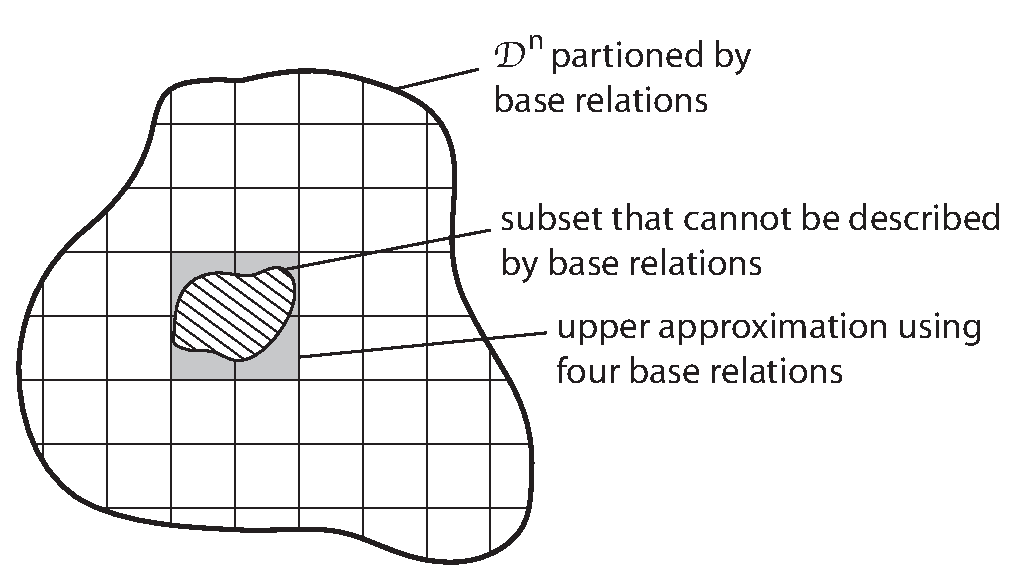
\includegraphics[scale=.5]{weak_op}}
	\caption{\label{FIG:weak-vs-strong} Illustration of a relation, i.e., a subset of $\mathcal{D}^n$, represented as an upper approximation}
\end{figure}

In the case of the weak  composition in a binary calculus $<\mathcal{B},\mathcal{D}^2>$ it is defined as:
$$
r \circ^{\star} s := \{ B \in \mathcal{B}\; |\; B \cap (r \circ s) \neq \emptyset \}
$$

Note that the use of an upper approximation of some operation still guarantees like in the case of strong operations that the empty relation can only be the result of contradicting information. However, the use of a weak operation can lead to situations in which a set of not agreeable statements is not detected as such.

Given that from a syntactical point of view the difference between weak and strong operations is not identifiable, \engine{} does not differentiate strong and weak operations syntactically.



%
%\subsection*{Operations of binary calculi}

%For binary calculi, two more operations are utilized. These
%are the \emph{converse} and \emph{composition} operations,
%we have already encountered above:

%\begin{description}
%\item[Converse:] $R^{\smallsmile} = \{\; (y,x)\; |\; (x,y) \in R\;\}$
%\item[Composition:] $R \circ S = \{\; (x,z)\; |\; \exists y \in D: \left((x,y) \in R \wedge (y,z) \in S\right)\;\}$
%\end{description}

%Again, here are two examples from the PA: The converse of $\{behind\}$ is
%$\{ahead\}$ and the composition of $\{ahead\}$ and $\{ahead,same\}$ is
%$\{ahead\}$ (if A is ahead of B and B is ahead or at the same level as
%C than A has to be ahead of C).

%For some calculi, the composition operation defined does not
%comply to the ``strong'' definition above, as this would
%result in a composition that is not closed for the set of
%relations $\mathcal{R}$ (and no finite set of relations including the base
%relations exists for which this is the case). In this case,
%the used composition operation is the
%``weak'' composition that takes the union of all base
%relations that have a non-empty intersection
%with the result of the strong composition:

%\begin{description}
%\item[Weak composition:] $R \circ_{weak} S = \{\; d\; |\; T \in \mathcal{BR} \wedge d \in T \wedge T \cap (R \circ S) \neq \emptyset\;\}$
%\end{description}
%For some calculi, it is not yet known whether the defined composition
%operation is ``strong'' or not.

%\section{Ternary calculi and their operations}
%\label{sec:ternops}

%While there is only one possibility to permute the two objects of a binary
%relation which leads to the converse operation, there exist 5
%such permutations for the three objects of a ternary relation.
%This results in the following 5 operations introduced in \citet{cosyzim96}:

%\begin{description}
%\item[Inverse:] $\mbox{INV}(R) = \{\; (y,x,z)\; |\; (x,y,z) \in R\; \}$
%\item[Short cut:] $\mbox{SC}(R) = \{\; (x,z,y)\; |\; (x,y,z) \in R\; \}$
%\item[Inverse short cut:] $\mbox{SCI}(R) = \{\; (z,x,y)\; |\; (x,y,z) \in R\; \}$
%\item[Homing:]   $\mbox{HM}(R) = \{\; (y,z,x)\; |\; (x,y,z) \in R\; \}$
%\item[Inverse homing:] $\mbox{HMI}(R) = \{\; (z,y,x)\; |\; (x,y,z) \in R\; \}$
%\end{description}

%It is in general not needed to specify all these operations as some can be expressed by others, but they are all available in \engine{} nonetheless.
%Composition for ternary calculi is defined accordingly to the binary case:

%\begin{description}
%\item[Composition:] $R \circ S = \{\; (w,x,z)\; |\; \exists y \in D: \left((w,x,y) \in R \wedge (x,y,z) \in S\right)\; \}$
%\end{description}
%
%Other ways of composing two ternary relations can be expressed as
%a combination of the unary permutation operations and the composition
%\citep{scivos01} and thus do not have to be defined separately and are
%also not accessible individually in \engine{}.
%The definition of weak composition is identical to the binary case.

%As we have not introduced a ternary calculus so far, we resign from
%giving any examples here, but some can be found later in Section
%\ref{sec:using-ri-engine}.

%\section{Conceptual neighborhoods}

\section{Checking Consistency}
\label{sec:consistency}

Determining consistency of a constraint network in which
the constraints are given as qualitative spatial relations
from a particular calculus, is a particular instance
of a \emph{constraint satisfaction problem} (CSP).
Unfortunately, the domains of our variables are typically
infinite (e.g.\ the set of all points in the plane) and
thus backtracking over all the values of the domain cannot
be used to determine consistency.

The techniques developed for relational constraint problems
are instead based on weaker forms of consistency called
\emph{local consistencies} which can be tested or enforced
based on the operations of the calculus and which are
under particular conditions sufficient to decide
consistency.

One important form of local consistency is \emph{path-consistency} which (in binary CSPs) means that for every triple of variables each consistent evaluation of the first two variables can be extended to the third variable in such a way that all constraints are satisfied. In the best case,
path-consistency decides consistency for a given calculus. This means, that
if we can make the network path-consistent by possibly removing some
base relations from the constraints without ending up with the empty relation,
we know that the original network is consistent. If this cannot be achieved,
the network has to be inconsistent. Unfortunately, it is usually not the case
that path-consistency decides consistency.

However, sometimes path-consistency is sufficient to decide consistency
at least for a subset $\mathcal{S}$ of the relations from $\mathcal{R}$,
for instance
the set of base relations. On the one hand, this means that whenever
our constraint networks only contains labels which are base relations,
we again can use path-consistency as a criterion to decide consistency.
On the other hand, if the subset $\mathcal{S}$ exhaustively splits
$\mathcal{R}$ (which means that every relation from $\mathcal{R}$ can be
expressed as a union of relations from $\mathcal{S}$), this at least
allows to formulate a backtracking algorithm to determine consistency
by recursively splitting the constraints and using path-consistency
as a decision procedure for the resulting CSPs with constraints from
$\mathcal{S}$ \citep{ladkin92_qualCSP}.

To enforce path-consistency, syntactic procedures called \emph{algebraic
closure algorithms} have been developed that are based
on the operations of the calculus (the composition operation in
particular) and work in $O(n^3)$
time for binary calculi and $O(n^4)$ for ternary calculi
where $n$ is the number of variables.
But again, we have to note
that these syntactic procedures do not necessarily yield the correct
results with respect to path-consistency as defined above.
Whether algebraic closure coincides
with path-consistency
needs be investigated for each calculus individually and we
again refer to the literature listed in the individual calculus descriptions
in Appendix \ref{sec:supp-spat-calc}.



\chapter{Using \engine}\label{sec:using-ri-engine}

\engine{} consists of a set of modules that logically structure
the different services provided, which will be explained below.
The general architecture is visualized in Fig.~\ref{fig:SparQ_Arch}.
The dashed parts are extensions planned for the future (see section
\ref{sec:outlook}).

\begin{figure}[ht]
 	\centering
	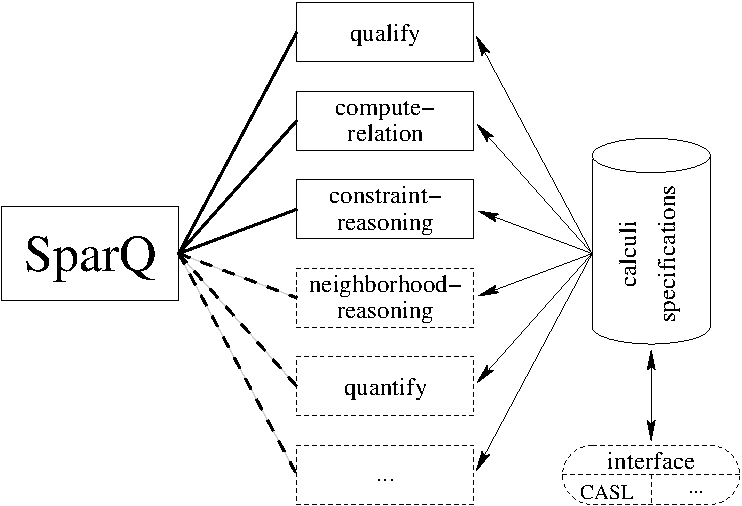
\includegraphics[width=0.6\textwidth]{SparQ_Structure}
	\caption{Module architecture of the SparQ toolbox.}
	\label{fig:SparQ_Arch}
\end{figure}

The general syntax for using \engine{}  is

\cmdline{./sparq <module> <calculus> <module specific parameters>}

where {\tt module} designates the particular module to use, {\tt calculus} refers to the qualitative calculus to use, and the remainder of the command line give command specific arguments which will be explained in the following. \engine{} can also be used in interactive mode (see section \ref{sec:interactive}) --- the general syntax is the same though.


\noindent Example:

\cmdline{./sparq compute-relation rcc-8 composition dc ntpp}

computes the composition of the rcc-8 relations $DC$ and $NTPP$. \engine{} prints the result {\tt (dc ec po tpp ntpp)} to the shell which stands for $\{DC, EC, PO, TPP, NTPP\}$.

%where `compute-relation' is the name of the module to be utilized, in this
%case the module for conducting operations on relations, `dra-24' is the
%\engine{} identifier for the dipole calculus \DRAc{}, and the rest are module
%specific parameters, here the name of the operation that should be conducted
%(`complement') and a string parameter representing the disjunction
%of the two dipole base relations \emph{lrll} and \emph{llrr}\footnote{Unions of base
%  relations are always represented as a space-separated list of the base
%  relations enclosed in parentheses in \engine{}.}. The example call thus computes the
%complement of the disjunction of these two relations.



\engine{} provides the following modules:

\begin{description}
\item[qualify] --- transforms a quantitative geometric description of a spatial configuration into a qualitative description based on one of the supported spatial calculi
\item[quantify] --- complement to qualify, computes an exemplary geometric model
\item[compute-relation] --- applies the operations defined in the calculi specifications (intersection, union, complement, converse, composition, etc.) to a set of spatial relations
\item[constraint-reasoning] --- performs computations on constraint networks
\item[neighborhood-reasoning] --- performs computations on constraint networks based on conceptual neighborhoods
\item[algebraic-reasoning] --- geometric reasoning using algebraic geometry
\item[analyze-calculus] --- relation-algebraic analysis of calculus structures
\end{description}

We will take a closer look at each of these three modules in the next sections.


\section{Command Line Options}\label{SEC:cmd-line-options}

Implemented switches:
\begin{description}
	\item[{\tt -v}] verbose mode primarily used for debugging purposes
	\item[{\tt -i, --interactive}] interactive mode (see section \ref{sec:interactive})
	\item[{\tt -p <port>, --port}] in interactive mode listen for connection on TCP/IP port rather using input from the shell
\end{description}


\section{General Syntax}\label{sec:syntax}

\engine{} is case-insensitive, so the notation {\em leftOf} and {\em Leftof} denote the same identifier. When printing, \engine{} uses small letters for relations and capital letters for objects.
There are some characters that must not be used in specifiers for either relations or objects, in particular parentheses ({\tt (},{\tt )}), punctuation ({\tt .}, {\tt ,}, {\tt ;}, {\tt :}), and {\tt \#} are not allowed. Nearly all other character sequences may be used---if in doubt, refer to the ANSI Common Lisp standard on symbols or just try out.


\subsection{Calculi Identifier}

\engine{} commands require specifying a calculus. For each calculus implemented in \engine{} an identifier has been defined (see the appendix for details on the calculi). Alternatively, calculi may be specified by giving the path name of the calculus definition file.

Calculi may have specific parameters, for example the granularity parameter in \opra{}. These parameters are appended with a `\verb|-|' after the calculus' base identifier. \verb|opra-3| for example refers to \opradrei{}. \pagebreak[4]

\renewcommand{\arraystretch}{1.5}
\begin{center}
\begin{longtable}{|p{4cm}p{6cm}ll|}\hline
	{\bf calculus identifier(s)} & {\bf calculus} & {\bf section} & {\bf page}\\ \hline \hline
%
	{\tt allen, aia, ia} & Allen's interval algebra \citep{allen83} & \ref{sec:allen} & \pageref{sec:allen} \\
	{\tt block-algebra, ba} & 2D block-algebra \citep{guesgen:89} & \ref{sec:block-algebra} & \pageref{sec:block-algebra} \\
	{\tt cardir} & Cardinal direction calculus \citep{ligozat98_carddir}  & \ref{sec:carddir} & \pageref{sec:carddir} \\
	{\tt depcalc, dep} & Dependency calculus \citep{Ragni05_DepCalc} & \ref{sec:depcalc} & \pageref{sec:depcalc} \\
	{\tt dipole-coarse, dra-24} & Dipole calculus \citep{moratz-renz-wolter-ECAI:00} & \ref{sec:dipole-coarse} & \pageref{sec:dipole-coarse} \\
	{\tt double-cross, dcc} & Double cross calculus \citep{cosyfre92} using the original tuple naming scheme & \ref{sec:double-cross} & \pageref{sec:double-cross} \\
	{\tt alternative-double- cross, adcc} & Double cross calculus \citep{cosyfre92} using the alternative single number naming scheme & \ref{sec:double-cross} & \pageref{sec:double-cross} \\
	{\tt flipflop, ffc, ff} & FlipFlop calculus \citep{Ligozat93_FlipFlopCalculus}& \ref{sec:flip-flop} & \pageref{sec:flip-flop} \\
	{\tt geomori, ori, align} & Geometric Orientation calculus & \ref{sec:geomoricalc} & \pageref{sec:geomoricalc} \\
	{\tt point-calculus, pc, point-algebra, pa} & Point algebra \citep{vilain_kautz_beek_89_constraint} & \ref{sec:pointcalc} & \pageref{sec:pointcalc} \\
	{\tt rcc-5} & Region connection calculus (RCC-5) \citep{randell92_rccb} & \ref{sec:rcc5} & \pageref{sec:rcc5} \\
	{\tt rcc-8} & Region connection calculus (RCC-8) \citep{randell92_rccb} & \ref{sec:rcc8} & \pageref{sec:rcc8} \\
	{\tt reldistcalculus} & Exemplary calculus from this manual & \ref{sec:calculus-spec} & \pageref{sec:calculus-spec}\\
	{\tt single-cross, scc} & Single cross calculus \citep{cosyfre92} & \ref{sec:single-cross} & \pageref{sec:single-cross} \\
	{\tt opra-} & Oriented point reasoning algebra (\opra{})\citep{moratz06_opra} & \ref{sec:opra} & \pageref{sec:opra}\\
	{\tt qtc-b11} & Qualitative trajectory calculus in 1D with distance \citep{Weghe04_PhD} & \ref{sec:qtc-b11} & \pageref{sec:qtc-b11}\\
	{\tt qtc-b12} & Qualitative trajectory calculus in 1D with velocity \citep{Weghe04_PhD} & \ref{sec:qtc-b12} & \pageref{sec:qtc-b12}\\
	{\tt qtc-b21} & Qualitative trajectory calculus in 2D with distance \citep{Weghe04_PhD} & \ref{sec:qtc-b21} & \pageref{sec:qtc-b21}\\
	{\tt qtc-b22} & Qualitative trajectory calculus in 2D with distance and velocity \citep{Weghe04_PhD} & \ref{sec:qtc-b22} & \pageref{sec:qtc-b22}\\
	{\tt qtc-c21} & Qualitative trajectory calculus in 2D with distance and side \citep{Weghe04_PhD} & \ref{sec:qtc-c21} & \pageref{sec:qtc-c21}\\
	{\tt qtc-c22} & Qualitative trajectory calculus in 2D with distance, side, and velocity \citep{Weghe04_PhD} & \ref{sec:qtc-c22} & \pageref{sec:qtc-c22}\\
	\hline
\end{longtable}
\end{center}
\renewcommand{\arraystretch}{1.0}


\subsection{Denoting Relations}
Relations are denoted using their name, as a disjunction using {\tt (}, {\tt )}, or by wild cards \verb=*= and \verb=?=.

\noindent Example using the RCC-8 calculus:\\
\begin{itemize}
	\item \verb=nttp=, \verb=Ntpp= both stand for the relation \verb=nttp=
	\item \verb=(nttp eq po)= stands for the relation \verb=nttp= $\cup$  \verb=eq= $\cup$  \verb=po=
	\item \verb=p?= stands for all relations with a two-letter name starting with 'p', i.e. \verb=po= $\cup$  \verb=pp= in case of the RCC-8 calculus
	\item \verb=*= stands for the universal relation
\end{itemize}

Please be aware, that if you pass arguments to \engine{} via the command line, the shell will perform some replacements, in particular if you are using parentheses or \verb=*=. You need to wrap quotes around your arguments, i.e. use \verb="(po eq)"= instead of \verb=(po eq)=, to avoid unwanted replacements.


\subsection{Denoting Configurations}
Configurations are static scene descriptions that interrelate named objects using qualitative relations of a particular calculus. Named objects are related by enclosing object identifiers and relation by parentheses, e.g. \verb=(A po B)=, configurations are specified using a list (enclosed in parentheses, no comma-separation), e.g. \verb=((A (po eq) B) (B eq C))=.

\section{Qualify}\label{sec:qualification}


The purpose of the qualify module is to turn a quantitative geometric scene
description into a qualitative scene description composed of base relations
from a particular calculus. The calculus is specified via the calculus
identifier that is passed with
the call to \engine{}. Qualification is
required for applications in which we want
to perform qualitative computations over objects whose geometric parameters
are known.

\begin{figure}[htp]
  \centering
  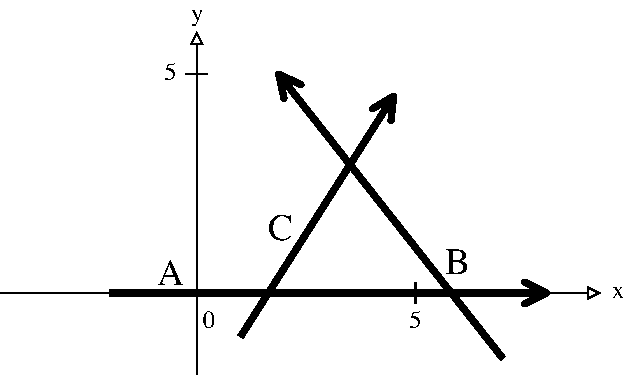
\includegraphics[width=.45\textwidth]{dipol-example}
  \caption{An example configuration of three dipoles.}
  \label{fig:dipol-example}
\end{figure}

The qualify module reads a quantitative scene description and
generates a qualitative description. A quantitative
scene description is a space-separated list of base object descriptions
enclosed in parentheses. Each base object description is a tuple consisting of
an object identifier and object parameters that depend on the type of the
object. For instance, let us say we are working with dipoles which
are oriented line segments. The object description of a dipole is of the
form `(name $x_s$ $y_s$ $x_e$ $y_e$)', where name is the identifier of this
particular dipole object and the rest are the coordinates of start
and end point of the dipole.
Let us consider the example in Fig.
\ref{fig:dipol-example} which shows three dipoles $A$, $B$, and $C$. The quantitative scene description for this
situation would be:

\begin{small}
\begin{verbatim}
( (A -2 0 8 0) (B 7 -2 2 5) (C 1 -1 4.5 4.5) )
\end{verbatim}
\end{small}

\noindent {\bf Note:} Coordinates may be specified as either integers (2; -3; ...), floats (3.2234; -1e-07), or rational numbers (13/7; -4/2). Using rational numbers can help avoiding effects of rounding errors. Depending on the basis entity (i.e., the domain of the qualitative calculus), different values need to be supplied. This table gives an overview:

\begin{center}
\begin{tabular}{|llp{7cm}|}\hline
	{\bf basis entity} & {\bf format} & {\bf semantics}\\ \hline \hline
	1d-point & {\tt (id x)} & Real-valued position of the point \\
	interval & {\tt (id s e)} & Real-valued (closed) interval\\
	2d-point & {\tt (id x y)} & Real-valued coordinates \\
	2d-oriented-point & {\tt (id x y dx dy)} & Real-valued coordinates and direction of the orientation\\
	dipole & {\tt (id xs ys xe ye)} & Directed line segment connecting the 2d points (xs ys) and (xe ye)\\
	2d-box & {\tt (id x1 y1 x2 y2)} & Axis-aligned rectangle with bottom left point (x1,y1) and top right point (x2,y2)\\
	polygon & {\tt (id x1 y1 ... xn yn)} & Polygon with vertices (x1,y1), (x2,y2), ... (xn,yn)\\
	\hline
\end{tabular}
\end{center}

The qualify module has one module specific parameter {\em mode} that needs to be
specified. It controls which relations are included into the qualitative scene description; there are two settings:

\begin{description}
	\item[{\tt all}] The relation between every object and every other object will be included. In the case of a binary calculus \engine{} prints out a configuration containing $n^2$ relations, if $n$ is the total number of  objects in the scene description.

	\item[{\tt first2all}] If mode is set to {\tt first2all} only the relations between the first and all other objects are computed in the binary case or between the first two objects and all other objects in the ternary case.
\end{description}

The resulting qualitative scene description is a space-separated list
of relation tuples enclosed in parentheses. A
relation tuple consists of an object identifier followed by a relation name
and another object identifier, meaning that the first object stands
in this particular relation with the second object.
%Thus, the qualitative
%scene description generated from the quantitative scene description above
%with the dipole calculus and  mode set to 'all' would be:
%
%\begin{small}\begin{verbatim}
%( (A rllr B) (A rllr C) (B lrrl C) )
%\end{verbatim}\end{small}
The command to produce the qualitative scene description
followed by the result is\footnote{In all the examples, input lines start with `\$'. Output of \engine{} is marked with `$>$'.}:

\shell{./sparq qualify dra-24 all "((A -2 0 8 0) (B 7 -2 2 5) (C 1 -1 4.5 4.5))"}{((A rllr B) (A rllr C) (B lrrl C))}

If we had chosen `first2all' as mode parameter the relation between $B$ and $C$ would not have been included in the qualitative scene description.

\section{Quantify}
The {\tt quantify} command complements the {\tt qualify} in the sense that it computes an exemplary geometric scene from a constraint network.

\shell{./sparq quantify allen "((a b b) (a fi c))"}{((C 1 2) (B 5 6) (A 3 4))}

\section{Compute-relation}


The compute-relation module allows to compute with the operations defined
in the calculus specification. The module specific parameters are the
operation that should be conducted and one or more input relations depending
on the arity of the operation. Let us say we want to compute the converse
of the \emph{llrl} dipole relation. The corresponding call to \engine{} and
the result are:

\shell{./sparq compute-relation dra-24 converse llrl}{(rlll)}

The result is always a list of relations as operations often yield
a disjunction of base relations. In this case, however, the disjunction
only contains a single relation.
The composition of two relations requires one more relation as parameter
because it is a binary operation, e.g.:

\shell{./sparq compute-relation dra-24 composition llrr rllr}{(lrrr llrr rlrr slsr lllr rllr rlll ells llll lrll)}

Here the result is a disjunction of 10 base relations. It is also
possible to have disjunctions of base relations as input parameters.
For instance, the following call computes the intersection of two
disjunctions:

\shell{./sparq compute-relation dra-24 intersection "(rrrr rrll rllr)"  "(llll rrll)"}{(rrll)}

Note that you need to put relation specifications in quotes when giving them
as arguments on the command line.
\engine{} can also process nested computations if individual parts are enclosed in parentheses, e.g., computing the complement of the converse of a relation can be done as follows:

\shell{./sparq compute-relation dra-24 "(complement (converse (rr??)))"}{(ells errs eses lere llll lllr llrl lrll lrrl lsel rele rlll rllr rrll rrlr rrrl rser sese slsr srsl)}

\noindent The following operations are currently implemented (see section \ref{sec:operations}):

\begin{longtable}{|l|p{8cm}|}
\hline
\multicolumn{2}{|l|}{\bf spatial:}\\ \hline
{\tt composition, comp} & $ (r, s) \mapsto r \circ s$\\
{\tt ternary-composition, tcomp}\ternaryonly & $ (r, s, t) \mapsto \bullet (r,s,t)$\\
{\tt n-ary-composition, ncomp}& $ (r_1, \ldots, r_n) \mapsto \bullet (r_1, \ldots, r_n)$\\
{\tt converse, cnv}\binaryonly & $r \mapsto r^{\smile}$ \\
{\tt homing, hm}\ternaryonly & $ r \mapsto hm(r)$\\
{\tt homingi, hmi}\ternaryonly & $ r \mapsto inv(hm(r))$\\
{\tt inverse, inv}\ternaryonly & $ r \mapsto inv(r)$\\
{\tt shortcut, sc}\ternaryonly & $ r \mapsto sc(r)$\\
{\tt shortcuti, sci}\ternaryonly & $ r \mapsto inv(sc(r))$\\[1ex]
\hline
\multicolumn{2}{|l|}{\raisebox{-2ex}[2ex][2.5ex]{{\bf calculi-theoretic:}}}\\ \hline
{\tt closure} & $ r_1 r_2 \ldots r_n \mapsto Cl(r_1,r_2,\ldots, r_n)$\newline
$Cl$ denotes the minimal set of relations that is closed under composition, converse,
and intersection\\
{\tt base-closure} & $Cl(br_1,br_2,\ldots , br_n)$\newline
Computes closure of the set of base relations\\
{\tt test-properties} & Tests whether a calculus meets relation algebra axioms\\
\hline
\multicolumn{2}{|l|}{\raisebox{-2ex}[2ex][2.5ex]{{\bf set-theoretic:}}}\\ \hline
{\tt complement, cmpl} & $ r \mapsto r^C$\\
{\tt minus} & $ r s \mapsto r \backslash s$\\
{\tt union} & $ r s \mapsto r \cup s$\\
{\tt intersection, isec} & $ r s \mapsto r \cap s$\\
\hline
\end{longtable}
\noindent Commands marked \binaryonly are valid for binary calculi only, commands marked \ternaryonly are valid for ternary constraints only. 

\note{The commands {\tt closure} and {\tt base-closure} are currently defined exclusively for binary calculi. The closure of a set of relations may be very large and computation may, consequently, take very long.}


%\section{Conceptual neighborhoods}

\section{Constraint-reasoning}\label{sec:constraint-reasoning}


The constraint-reasoning module reads a description of a constraint
network---which is a
qualitative scene description that may include disjunctions and may be
inconsistent and/or underspecified---and performs an operation on it,
e.g., a particular kind of consistency check:
%\footnote{The constraint-reasoning
%module also provides some
%basic actions to manipulate constraint networks that are not further
%explained in this text. One example is the `merge' operation that is
%used in the example in Section \ref{sec:integration}.}.
\begin{center}
{\verb= constraint-reasoning <calculus> <operation> <constraint-network> ... = }
\end{center}

%Which type of operation is executed depends on the first module specific parameter. 
Currently, operations are implemented for
checking consistency of a constraint network and propagating constraints
(`check-consistency', `algebraic-closure', `ternary-closure', `scenario-consistency'),
for manipulating constraint networks (`refine', `extend', `update') and
for correspondence between two networks (`match', `best-match').
%`consistency' `algebraic-closure', `scenario-consistency', `refine'\footnote{In former
%  versions of \engine{}, the `refine' action was called `merge'. This naming
%is still valid for backward compatibility reasons but may vanish in the future.}  and `extend'.

%\begin{description}
%\item [action] --- The actions currently provided are `consistency', `algebraic-closure', and
%`scenario-con\-sis\-ten\-cy' which determine which kind of consistency check is
%performed, as well as `refine' and `extend' which perform set operations on
%constraint networks.
%\end{description}
\subsection{Constraint-based reasoning}
Action `algebraic-closure' causes the module to
enforce path-consistency on the constraint network using
a variant of 
Mackworth's AC-3 algorithm \citep{mackworth77}. As a result the constraint network
obtained is returned. 
If during constraint propagation an inconsistency is discovered, the inconsistency is reported and not netwrok is returned.
In case of ternary calculus the canonical extension
of the AC-3 algorithm as described in \citet{cosy:dylla:2004:tpcc_complexity}
is used. 
For ternary calculi there also exist the option to use the more natural ternary composition operation (if defined for the respective calculus) instead of the binary composition operation.
Enforcing path-consistency using ternary composition operation is invoked using `ternary-closure'.

\subsection*{Examples}

We could for instance check if the
scene description generated by the
qualify module in Section \ref{sec:qualification} is algebraically closed---which of course it is.
To make it slightly more interesting, we add the base relation \emph{ells} to the
constraint between $A$ and $C$ resulting in a constraint network that is not
algebraically closed:

\shell{./sparq constraint-reasoning dra-24 algebraic-closure\\  "((A rllr B) (A (ells rllr) C) (B lrrl C))"}
{Modified network.\\ > ( (B (lrrl) C) (A (rllr) C) (A (rllr) B) )}

The result is an algebraically closed constraint network in which \emph{ells} has been
removed. The output `Modified network' indicates that the original network was not
algebraically closed and had to be changed. Otherwise, the result would
have started with `Unmodified network'.
In the next example we remove the relation \emph{rllr} from the disjunction
between $A$ and $C$.  This results in a constraint network for which algebraic
closure detects an inconsistency which means it is not globally consistent.

\shell{./sparq constraint-reasoning dra-24 algebraic-closure\\  "((A rllr B) (A ells C) (B lrrl C))"}
{Not consistent.\\ > ((B (lrrl) C) (A () C) (A (rllr) B))}

\engine{} correctly determines that the network is inconsistent and returns
the constraint network in the state in which the inconsistency showed up
(indicated by the empty relation () between $A$ and $C$).

In a last example for algebraic-closure we use the ternary double cross calculus:

\shell{./sparq constraint-reasoning dcc algebraic-closure\\  "((A B (7\ul 3 6\ul 3) C) (B C (7\ul 3 6\ul 3 5\ul 3) D) (A B (3\ul 6 3\ul 7) D))"}{Not consistent.\\ > ((A B (3\ul 6 3\ul 7) D)(A B () C)(B C (5\ul 3 6\ul 3 7\ul 3) D)(D C (0\ul 4 1\ul 5 2\ul 5 3\ul 5 3\ul 6 3\ul 7 4\ul 4 5\ul 3 6\ul 3 7\ul 3 b\ul 4) A))}

%((A B (3\ul 6  3\ul 7) D) (A B (6\ul 3 7\ul 3) C) (B C (5\ul 3 6\ul 3 7\ul 3) D) (D C () A))}


If `scenario-consistency' is provided as argument, the constraint-reasoning
module checks if an algebraically closed scenario exists for the given network.
It uses a backtracking algorithm to generate all possible
scenarios and checks them via algebraic closure as described above. Knowledge about tractable sets, if defined for the calculus at hand, are exploited too.
A second module specific parameter determines what is returned as the result of the search:

\begin{description}
\item [return] --- This parameter determines what is returned in case of a constraint
network for which path-consistent scenarios can be found. It can take
the values `first' which returns the first path-consistent
scenario, `all' which returns all path-consistent scenarios, and
`interactive' which returns one solution and queries whether the search shall be continued. Finally,  `check' instructs \engine{} to only check existence of an algebraically closed scenario which, in some cases, can be much faster than actually computing a solution.
\end{description}

While computing scenario-consistency, algebraic closure is also used as a
forward-checking method during the search to make it more efficient.
For certain calculi, the existence of an algebraically closed scenario
implies consistency.
However, this again has to be investigated for each calculus (cmp. Section \ref{sec:consistency}).

In the following example, we use `first' as
additional parameter so that only the first solution found is returned:

\shell{./sparq constraint-reasoning dra-24 scenario-consistency first\\
 "((A rele C) (A ells B) (C errs B) (D srsl C) (A rser D) (D rrrl B))"}
{((B (rlrr) D) (C (slsr) D) (C (errs) B) (A (rser) D) (A (ells) B) (A (rele) C))}

In case of an inconsistent constraint network, \engine{} returns
`Not consistent.' as in the following example:

%\marginpar{example needs to be complemented.}

\shell{./sparq constraint-reasoning dra-24 scenario-consistency first\\
 "((A rele C) (A ells B) (C errs B) (D srsl C) (A rser D) (D rllr B))"}
{Not consistent.}

For calculi which define tractable subsets the consistent scenarios may be
printed in a condensed form by giving disjunctions of  base relations such
that all combinations determine a consistent scenario, e.g.

\shell{./sparq constraint-reasoning rcc8 scenario-consistency all\\ "((a po b) (b ntpp c))"}
{((B (ntpp) C)(A (ntpp po tpp) C)(A (po) B))\\
> 3 scenarios found, no further scenarios exist.}

In this example, any of the relations $ntpp$, $po$, $tpp$ holding between $A$ and $C$ describes
a consistent scenario, thus there are three scenarios in total.

%$
\subsection{Manipulating constraint networks}
Constraint network manipulation is realized by operations which compute the conjunction of two constraint networks.
With qualitative calculi it is natural to assume that a constraint network that does not define a constraint between two objects (or which does not even involve the objects) implicitly declares the universal relation as constraint. 
This allows manipulation with three simple operations.

The action 'refine' returns the conjunction of two constraint
networks. Analogously, 'extend' returns the disjunction:

\shell{./sparq constraint-reasoning dra-24 refine "((A (rele errs) B))" "((A errs B))"}
{((A errs B))}

\shell{./sparq constraint-reasoning dra-24 extend "((A rele B))" "((A errs B))"}
{((A (rele errs) B))}

Finally, operation `update' allows constraints to be overwritten:

\shell{./sparq constraint-reasoning dra-24 update "((A rele B) (B eses C))" "((B llrr C))"}
{((B (LLRR) C) (A (RELE) B))}



Overview of commands operating on constraints:
\begin{longtable}{|p{4.5cm}|p{9cm}|}
\hline
\multicolumn{2}{|l|}{\bf consistency checking:}\\ \hline
{\tt check-consistency} & decides consistency using calculus-specific consistency check\\[0,5ex]
{\tt algebraic-closure}, {\tt a-closure}, {\tt path-consistency}  & Enforces path-consistency --- since this is a purely syntactical operation on the
					level of qualitative relations the term ``algebraic closure'' is more adequate.
					However, since ``path-consistency'' is widely used in this meaning, this name is
					supported too.\\[0,5ex]
{\tt scenario-consistency} & Computes algebraically closed networks containing base-relations only\\[0,5ex]
{\tt ternary-closure} & Computes algebraically closed networks using ternary composition with ternary calculi\\[0,5ex]
{\tt match} & Computes possible correspondence (isomorphy and joint consistence)\\[0,5ex]
%{\tt best-match} & Interactively computes possible correspondence (isomorphy and joint consistence)\\[1,0ex]
\hline
\multicolumn{2}{|l|}{\raisebox{-2ex}[2ex][2.5ex]{{\bf manipulating constraint networks:}}}\\[0,5ex] \hline
{\tt refine} & Merges two networks by intersecting corresponding constraints\\[0,5ex]
{\tt extend} & Merges two networks by uniting corresponding constraints\\[0,5ex]
{\tt update} & Merges two networks by overwriting corresponding constraints\\ \hline
\end{longtable}

\section{Algebraic reasoning}\label{sec:a-reasoning}
\engine{} includes a module for reasoning about real-valued domain using techniques of algebraic geometry. Spatial reasoning problems get posed as algebraic problems of solving systems of equations. The techniques implemented in \engine{} are based on Gr\"obner bases (see e.g., \cite{cox:98}). The main service offered by the algebraic reasoning module is to provide a consistency checking mechanism for constraint networsk that is based on the relation semantics only. This means, algebraic reasoning can be used to compute or to verify operation tables such as e.g., used for specifying the composition operation. Furthermore, algebraic reasoning can be used to analyze certain calculi properties.

\medskip

\subsection{Consistency checking}
The algebraic reasoning module provided consistency analysis of constraint networks using the same syntax as constraint based consistency analysis (see Sec.~\ref{sec:constraint-reasoning}). In contrast to constraint based reasoning, algebraic reasoning only makes use of an algebraic relation specification.

\cmdline{./sparq a-reasoning <calculus> consistency <network>}

Networks are denoted as defined in the context of the constraint based reasoning  module.
Possible results:
\begin{description}
	\item[{\tt SATISFIABLE}] The network is proven to be satisfiable.
	\item[{\tt NOT SATISFIABLE.}] The network is proven to be unsatisfiable.
	\item[{\tt CANNOT DECIDE.}] Neither one of the above proofs succeeded.
\end{description}

Currently, the implementation of the algebraic reasoning module aims at proving inconsistency of constraint networks, thus the answer ``satisfiable'' appears only rarely. Making algebraic reasoning a more powerful tool is ongoing research.

\noindent Example:\\ \noindent
\cmdline{sparq -v a-reasoning ff consistency  "((A B l C) (B C l D) (A B f D))"}

By turning on the verbose mode (command line option ``{\tt -v}''), the proof generated by \engine{} is printed to the console. Algebraic reasoning as implemented in \engine{} is based on analyzing Gr\"obner bases. Computing Gr\"obner bases is a computationally very expensive process and a time limit is implemented into \engine{} to prevent hangs. Currently, the time limit is hard wired to approx.~17 minutes. To abort an ongoing computation, use Control-C to stop \engine{}. Currently, the time limit is a compile-time option, hence, to increase time limit, your need to change the source parameter declaration {\tt *timeout*} in the beginning of {\tt Source/polysolver.lisp}. Note that the unit size is ms here.

Due to the computational demands of algebraic reasoning we advice users to utilize this method only for analyzing small constraint networks. The most useful application of this module is for computing calculus operations. 

\subsubsection*{Example: computing calculus operations}
Suppose, you are about to introduce a new qualitative calculus and have designed the set of base relations. In order to do any constraint based reasoning with this new calculus, permutation operations (converse, inverse, shortcut, etc.) and the composition operation need to be defined. Determining composition operation tables is a demanding process: all 3-consistent constraint networks involving $k+1$ base objects need to be computed whereby $k$ denotes the arity of the calculus. In such situations algebraic reasoning can be effectively applied to rule out inconsistent networks. Consider again the example from above, analyzing the constraint network 
\begin{center}
	{\tt ((A B l C) (B C l D) (A B f D))}
\end{center}
in context of the FlipFlop base relations (see \ref{sec:flip-flop}) \engine{} will come up with the reply that the given network is not consistent. Therefore, the relation ``f'' (front) is not a possible result of the composition of ``l'' and ``l'' (left). To automate operation analysis an additional command is implemented.

\subsection{Operation analysis}
This command applies algebraic reasoning to check operations as explained in the previous section.

\cmdline{sparq a-reasoning <calculus> analyze-operation <operation>}

The command iterates over all base relations to analyze the given operation (e.g., composition, shortcut, etc.) and prints out a table summarizing the results. The table for an unary operation looks like this:
\begin{verbatim}
progress. r        analysis
......... r1        Verified.
......... r2        CANNOT INCLUDE: (r1)
......... r3        could not prove non-membership of : (r1 r2)
......... r4        could not prove membership of : (r2)
......... r5        ALSO INCLUDES: (r1)
\end{verbatim}

The dots in the progress column are printed to show the progress of the verification, the column labeled ``r'' lists the relation examined. The column analysis lists the result which is one of the following:
\begin{description}
	\item[{\tt Verified}] The entry of the operation table as given in the calculus specification has been verified.

	\item[{\tt CANNOT INCLUDE (r1 r2 ...)}] The reported base relations are listed in the operation table but they cannot be the result of applying the operation. This is an error in the operation table - remove the conflicting relations.
	
	\item[{\tt ALSO INCLUDES: (r1 r2 ...)}] The reported base relations have been proved to be missing in the operation table - add them.

	\item[{\tt could not prove membership of: (r1 r2 ...)}] The reported base relations are listed in the operation table, but no proof could be generated to show that these relations can be the result of applying the operation to $r$. This does not indicate an error in the operation table.

	\item[{\tt could not prove non-membership of: (r1 r2 ...)}] The reported base relations are not listed in the operation table, but no proof could be generated to show that these relations cannot be the result of applying the operation to $r$. This does not indicate an error in the operation table.
\end{description}

\subsection{Qualification}
When an algebraic calculus specification is provided, it can be used in qualification too. This means, a scenario can be qualified without supplied an designated qualification function.

\cmdline{./sparq a-reasoning <calculus> qualify <option> <scenario>} 

Syntax and options are the same as for the qualification module described in Sec.~\ref{sec:qualification}.

\section{Analyzing Calculi}\label{sec:analyze-calculus}
\engine{} involves a set of commands that aim to aid researchers to analyze qualitative calculi. 
These commands are summarized in the module {\tt analyze-calculus} and are named as follows:
\begin{description}
	\item[{\tt test-algebra}] Using this command one can check whether a calculus definition meets the axioms that define a relation algebra in the sense of Tarski. The command is also helpful to identify potential errors in operation tables of newly added calculi---if \engine{} only reports very few violations of an axiom, these violations may be caused my en erroneous entry in an operation table
	
	\item[{\tt test-property}] This command allows specific properties or axioms to be tested for a specific calculus. 
	Essentially, \engine{} checks a single statement as usable with the {\tt compute-relation}-command with quantified variables. 
	We illustrate this by an example, checking whether {\tt rrc5} has an idempotent converse operation:
	\cmdline{./sparq analyze-calculus rcc5 test-property "(forall r baserel) (equals r (converse (converse r)))"}
	Here, {\tt} is a variable ranging over all base relations of the RCC-5 calculus. 
	Note that the quotes are necessary to prevent a Unix shell from interpreting parenthesis expressions.
	It is possible to use quantifiers {\tt exists} and {\tt forall}, ranging over either base relations ({\tt baserel}) or all general relations ({\tt rel}). 
	Special operators for comparing relations that are likely used with this command are {\tt equal, covers, coverseq} (either {\tt equal} or {\tt covers} hold), {\tt coveredBy, coveredByEq}.
	

	\item[{\tt algebra-stats}] Operation tables of calculi often differ in their information content, e.g., how often a universal relation occurs as the result of applying a composition operation. This command determines the information content of applying $k$ steps of composition, an additional parameter determines the time in seconds to spend on analyzing the calculus.
	
\end{description}

\section{Neighborhood-Based Reasoning}\label{sec:cnh}
The aim of this module is to provide tools for reasoning based on the notion of conceptual neighborhood \citep{cosyfre92a} that can be used for addressing spatial change over time as well as constraint relaxation. 


TBD

\begin{table}
\begin{tabular}{lp{7.5cm}}
\toprule
\multicolumn{2}{l}{\tt neighborhood-reasoning <CALCULUS> <NEIGHBORHOOD> ...}\\
{\tt \small similarity OP <CSP> <CSP>} & computes similarity of two constraint-networks, using OP as distance accumulation operation\\
{\tt \small neighbors <REL> } & gives the conceptual neighbors of a relation\\
{\tt \small merge OP OP <CSP> <CSP} & merges two constraint networks, using OP as distance accumulation operation\\
{\tt \small relax <RELATION>} & coarsens relation by including all conceptual neighbors of a relation\\
{\tt \small neighborhood-distance <REL> <REL> } & distance in the neighborhood graph\\ 
\bottomrule
\end{tabular}
\caption{\label{tab:cnh-commands}Summary of commands for neighborhood-based reasoning}
\end{table}

\section{Interfaces}\label{sec:interfaces}

Currently, \engine{} provides only means for exporting calculi specification to formats used in other reasoners, the syntax is as follows:

\cmdline{./sparq export <calculus> <type> <filename>}

where type is one of
\begin{description}
	\item[{\tt qat}] QAT is a toolkit for qualitative spatial and temporal reasoning written in Java \citep{Condotta_Ligozat_Saade_06_A} that uses an xml format for calculi specifications. Currently, only binary calculi can be exported into this format. For more information see:\\ \verb=http://www.cril.univ-artois.fr/~saade/QAT=
	\item[{\tt gqr}] GQR is a generic constraint reasoner for binary calculi, i.e., it provides an alternative implementation of \engine{}'s constraint-reasoning module but limited to binary calculi. For more information see:\\ \verb=https://sfbtr8.informatik.uni-freiburg.de/R4LogoSpace/Resources/GQR=
\end{description}

By invoking the export command, \engine{} creates a file \verb=<filename>= (two in the case of GQR export) in \engine{}'s main directory.


\section{Interactive Mode}\label{sec:interactive}

\engine{} can be started in interactive mode to process commands repeatedly. This greatly reduces
overhead of loading the program or calculi definitions. Interactive mode is activated by the command line option {\tt -i} (or {\tt --interactive}). The command syntax is identical to the standard mode of operation, there are some additional commands though:\pagebreak[4]

\begin{center}
\begin{longtable}{|lp{9cm}|}\hline
	{\bf command} & {\bf description} \\ \hline \hline
	{\tt quit} & exits \engine{}\\
	{\tt help} & prints short help message\\
	{\tt load-calculus CALC} & loads a specified calculus into memory\\
	{\tt *} & used as calculus specifier in commands, {\tt *} stands for the calculus recently loaded into memory. This avoids overhead of reloading a calculus\\
	{\tt let VAR = EXP} & binds expression/result of command to variable\\
	{\tt let (VAR1 ... VARN) = EXP} & bind multiple variables to commands providing multiple return values\\
	{\tt print \$VAR} & print value bound to variable\\
	 \hline
\end{longtable}
\end{center}

\subsection{Variables}
In the interactive mode, \engine{} provides simple variables to reduce typing effort -- or network traffic, if \engine{} is interfaced using sockets. 
Variables are set using the {\tt let} command; {\tt print} allows values to be printed out. 
As some commands return multiple values, {\tt let} allows multiple variables to be bound at once, the special name \verb=_= (underscore sign) can be used to ignore a value.
When used in commands, variables are marked by a leading dollar sign. Note that names are case insensitive. Here is an example on using variables:

\outp{SparQ> let myScene = qualify pc all ((a 1) (b 2) (c 1/4))\\
> ((A < B) (A > C) (B > C))\\[0.5ex]
SparQ> let myNeWScene = constraint-reasoning pc extend \$myscene ((a < d))\\
> ((A (<) B) (A (>) C) (A (<) D) (B (>) C))\\[0.5ex]
SparQ> let (\_ closedNet) = constraint-reasoning pc a-closure \$myNewScene\\
Modified network.\hfill{\it ;; ignore first return value}\\
((B (>) C)(D (>) C)(D (< = >) B)(A (>) C)(A (<) B)(A (<) D))\\[0.5ex]
SparQ> constraint-reasoning pc scenario-consistency first \$myNewScen\\
((D (>) A)(C (<) A)(C (<) D)(B (>) A)(B (>) D)(B (>) C))\\[0.5ex]
SparQ> print \$myScene\\
> ((A < B) (A > C) (B > C))}

 % 
\section{Including \engine{} Into own Applications}\label{sec:integration}

In interactive mode, \engine{} can be used as server that can easily be integrated
into own applications. We have chosen a client/server approach as it allows
for straightforward integration independent of the programming language used
for implementing the application.

When run in server mode, \engine{} uses a
TCP/IP connection as input/output and interacts with the client via simple plain-text
line-based communication. This means the client sends commands just like if using
\engine{} in interactive mode, and can then read the results from the TCP/IP stream.

\engine{} is started in server mode by providing the command line option
\verb|--interactive| (\verb|-i|), optionally followed by \verb|--port| (\verb|-p|) to specify the port.

\cmdline{./sparq --interactive --port 4443}

If no port is given, \engine{} interacts with standard-input and
standard-output, i.e., it can
be used interactively from the shell.

%\lstset{language=Python}

\lstinputlisting[basicstyle=\footnotesize\tt,language=Python,float=t,caption={Integrating \engine{} into own applications:
  an example in Python.},label={fig:python-example},firstnumber=1]{python-integration.py}

%$
An example of client/server communication with \engine{} is given in Listing
\ref{fig:python-example} which shows a small Python script
%\footnote{Special care may be given to line endings, depending on
%  the operating system. Refer to the user manual for further details.}
 that opens a connection to the server and performs some simple
computations (qualification, adding another relation, enforcing
algebraic closure). It produces the following output:

\outp{> ((A rrll B) (A rrll C))\\
> ((A rrll B) (A rrll C) (B eses C))\\
> Not consistent.\\
> ((B (eses) C) (A (rrll) B) (A () B))}

Special care may be given to line endings, depending on the operating
system. The example code defines a function to strip line endings from the
result lines. Furthermore, comment lines beginning with a semicolon have to be
ignored. Also note that every first return line after a command comes with a
preceeding \verb|sparq| prompt, so the first six characters are stripped of the
result. This behavior is due to compatibility reasons and will definitely change
in later versions of \engine{} (downward compatibility, however, will be granted).


\section{Adding new Calculi}

For most calculi it should be rather easy to include them
into \engine{}. Adding a new calculus consists of two steps:

\begin{enumerate}
	\item Provide a calculus specification and store it in \engine{}'s subdirectory {\tt Calculi}
	\item Register your calculus in the calculus registry {\tt Calculi/calculus-registry.lisp}
\end{enumerate}

\engine{} also allows loading calculi from an arbitrary file (by supplying the path name as calculus argument), so calculi are not required to be registered permanently. Example:

\cmdline{./sparq compute-relation /path/to/my/calculus.lisp converse someRel}

\subsection{Calculus Specification}\label{sec:calculus-spec}

Let us start by giving an example for a simple calculus for
reasoning about distances between three point objects that distinguishes only the three relations `closer', `farther', and `same'. Following the intuition, $A\, B\, \text{\tt closer}\, C$ holds if and only if $A$ and $B$ are closer to one another than $A$ is to $C$. Farther and same are defined analogously.
Listing \ref{fig:specification-reldist} shows the specification which is done in Lisp-like syntax.

\lstset{language=LISP}
\lstinputlisting[float=htp,caption={Specification of a simple ternary calculus for reasoning about
  distances.},label={fig:specification-reldist},firstnumber=1]{specification.lisp}

The arity of the calculus, the base relations, the identity relation and the
different operations have to be specified, using lists enclosed in parentheses
(e.g.\ when an operation returns a disjunction of base relations). In this
example, the shortcut operation applied to `same' yields `same' and composing
`closer' and `same' results in the universal relation written as the disjunction
of all base relations. It is not required to specify the inverse shortcut and inverse homing operations (cmp. Section \ref{sec:operations}) as these can be computed by applying the other operations (e.g., inverse
of shortcut yields inverse shortcut). It is, principally,
possible to leave more operations unspecified. However, this may mean that certain computations cannot be performed for this calculus.

In addition to the calculus specification, one could provide the
implementation of a qualifier function which for a n-ary calculus takes n geometric objects of the corresponding base type as input
and returns the relation holding between these objects. The qualifier
function  encapsulates the methods for computing the qualitative relations
from quantitative geometric descriptions.
If it is not provided, the qualify module will not work for this calculus.

For some calculi, it is not possible to provide operations in form of simple
tables as in the example. For instance, \opra\ has an additional parameter that specifies the granularity and  influences the number of base relations.  Thus, the operations can only be
provided in procedural form, meaning the result of the operations are
computed from the input relations when they are required. For these cases,
\engine{} allows to provide the operations as implemented functions and
uses a caching mechanism to store often required results.

\subsection{Specification Reference}

Any specification must be in the form

\begin{verbatim}
(def-calculus <NAME>
  {<SLOT-AND-OPTIONS>}* )
\end{verbatim}
where \verb=<NAME>= is a textual description of the calculus enclosed in double quotes. \linebreak[4]
\verb=<SLOT-AND-OPTIONS>= refers to a collection of calculus properties (in no particular order) that consists of pairs of a so-called slot specifier (always starting with a colon) and slot-specific options. Table \ref{TAB:slots-in-calc-def} gives an overview. The abbreviations {\tt SRC} and {\tt LIB} stand for source code specification and library link which are explained thereafter.

\begin{table}
\rotatebox{90}{%
\begin{tabular}{|lp{6cm}p{8cm}|}
\hline {\bf slot} & {\bf arguments} & {\bf description} \\ \hline \hline
{\tt :arity} & {\tt :binary$|$:ternary} & arity of the calculus\\
{\tt :base-relations} & {\tt (r \{r-i\}$^*$) $|$ LIB $|$ SRC} & list of base relations\\
{\tt :identity-relation} & {\tt r} & relation $r$ that holds in $A\, r\, A$\\
{\tt :consistency} & {\tt method} & method for deciding consistency, one of {\tt :a-closure, :n-ary-closure, :scenario-consistency, :a-consistency, :n-ary-scenario-consistency}\\
{\tt :converse-operation} & {\tt(\{(r1 r1-cnv)\}$^*$) $|$ LIB $|$ SRC} & lists of relations and their corresponding converse relation, reference to external library function, or Lisp code\\
{\tt :inverse-operation} & 	{\tt(\{(r1 r1-inv)\}$^*$) $|$ LIB $|$ SRC} & lists of relations and their corresponding inverse relation, reference to external library function, or Lisp code\\
{\tt :shortcut-operation} & {\tt(\{(r1 r1-sc)\}$^*$) $|$ LIB $|$ SRC} & lists of relations and their corresponding shortcut relation, reference to external library function, or Lisp code\\
{\tt :homing-operation} & {\tt(\{(r1 r1-hm)\}$^*$) $|$ LIB $|$ SRC} & lists of relations and their corresponding homing relation, reference to external library function, or Lisp code\\
{\tt :composition-operation} &  {\tt(\{(r1 r2 r1r2-cmp)\}$^*$) $|$ LIB $|$ SRC} & lists of two relations and their composition, reference to external library function, or Lisp code\\
{\tt :n-ary-composition-operation} &  {\tt(\{(r1 r2 ... rn r-cmp)\}$^*$) $|$ LIB $|$ SRC} & lists of n relations and their composition, reference to external library function, or Lisp code\\
{\tt :basis-entity} & {\tt :1d-point $|$ :interval $|$ :2d-point $|$ :dipole $|$ :2d-oriented-point $|$ :2d-box} & type of the basis objects, domain of the calculus\\
{\tt :parametric?} & {\tt t $|$ nil} & Boolean whether the calculus depends on a parameter or not\\
{\tt :qualifier} & {\tt :algebraic $|$ SRC $|$ LIB} & qualifier specification ({\tt :algebraic} is not yet fully functional)\\ \hline
\end{tabular}}
\caption{\label{TAB:slots-in-calc-def} Overview of the slots in calculi definitions and their options}
\end{table}

\subsection{Operation Specification}

Calculi comprise the definition of operations like converse or composition for which \engine{} provides three principles ways of specification:
\begin{enumerate}
	\item Tabular form (suits most standard calculi)
	\item Lisp source code
	\item Reference to C function in external library
\end{enumerate}

The tabular form is straight-forward. In the case of a unary operation (such as e.g., converse) it is simply a space-separated list of lists that give a relation and the respective outcome when applying the operation. Note that the operation needs only to be defined for base relations! In the case of the binary composition operation the tabular form is a list of lists that give the result for any combination of two base relations.

The last two options of operation specification are particular relevant for defining a quantifier or defining parametrical calculi, i.e., calculi that are instantiated by some parameter(s). In \engine{}, these calculi use identifiers that end with a minus ``{\tt -}'', e.g., {\tt opra-}.


\subsubsection{Lisp source operation specification}

Definitions may be supplied as Lisp function which then will be compiled by \engine{}. Lisp functions need to be denoted as lambda expressions. Here is an (slightly silly) example for specifying base relations by a Lisp function:

\begin{verbatim}
:base-relations #'(lambda () (list 'closer 'farther 'same))
\end{verbatim}

As can be observed, relations are simply returned as lists of relations and symbols are used to represent base relations. When specifying an operation that requires an input parameter to the function (e.g., converse, composition), then these are the arguments passed to the provided function. If a parametric calculus is defined, then the parameter will be accessible in by the globally visible parameter {\tt calculi:*calculus-parameter*}.

Altogether, the exemplary specification from above is equivalent to

\begin{verbatim}
:base-relations (closer farther same)
\end{verbatim}

{\bf Note:} Though you must use lambda expressions to specify lisp functions, you may define additional functions or parameters in the calculus definition. As the Lisp programmer would expect, the calculus definition is processed by the Lisp compiler and {\tt def-calculus} is a (quite complex) compiler macro.

\subsubsection{Lisp source qualifier specification}

Providing a lisp source definition for qualifiers is similar to specifying operations. In the case of a binary calculus you need to provide a 2-argument function, in the case of a ternary calculus a 3-argument function. These arguments are exactly those of the command qualify but without the object identifier, i.e., a qualifier for the point-based calculus (e.g., cardinal directions) requested by the command "qualify cardir ((A 2 3)  (B 1 3) (C -3 2))" will lead to calls passing the lists {\tt (2 3)}, {\tt (1 3)}, or {\tt (-3 2)} as arguments. Supplied functions are not required to do any error checking, as this is taken care of already.


\subsubsection{External operation libraries}

All operations may be specified by giving a reference to an external library by writing \verb=(external-lib LIBNAME C_FUNC)=. Hereby, \verb=LIBNAME= must be a string (delimited by double quotes) referring to a shared library inside \engine{}'s subdirectory {\tt Lib/bin}, \verb=C_FUNC= (a string too) gives the name of the corresponding C function to call. In principal, any programming language can be used as long as it allows for building a shared library that provides functions that follow the C calling convention. The signature of the C function for unary operations must be

\begin{verbatim}
	const char* C_FUNC( const char* param, const char* relation)
\end{verbatim}

When called by \engine{}, \verb=C_FUNC= is passed the currently active calculus parameters (ignore, if your calculus does not use parameters), i.e., all characters that are appended to the last ``-'' in the calculus name. As second argument, the relation is passed. The function needs to return the result in the same form \engine{} uses as print form for relations. In case of returning disjunctions, this means a space-separated list enclosed in parentheses.

When defining a binary operation (composition), the signature looks as follows:

\begin{verbatim}
	const char* C_FUNC( const char* param, const char* r1, const char* r2)
\end{verbatim}

Obviously, two relations need to be passed to the composition operation.

\subsubsection{External qualifier libraries}

Similar as with operation specification, external libraries can be used for defining
a qualifier module for \engine{}. The signature of the external functions is as
follows:

\begin{verbatim}
	const char* C_FUNC( const char* param, double P1, double P2, ...)
\end{verbatim}

Put differently, \engine{} passes (besides the calculus parameter) all spatial information as double precision floats to the function. The amount of parameters depends on:
\begin{itemize}
	\item the arity of the calculus
	\item the dimension of the calculus' basis entities
\end{itemize}

Let $a$ denote the arity of a calculus (either $a=2$ or $a=3$) and let $d$ denote the dimension of the basis entity, then $a\cdot d$ double parameters are passed. Dimensions of currently supported basis entities are as follows:

\begin{center}
\begin{tabular}{|ll|}\hline
	basis entity & $d$\\ \hline \hline
	1d-point & 1\\
	interval & 2\\
	2d-point & 2\\
	dipole & 4\\
	2d-oriented-point & 4\\
	2d-box (axis aligned rectangle) & 4 \\
	polygon & $2\times$ number of vertices
	\\ \hline
\end{tabular}
\end{center}

\medskip
{\bf Limitations:} Passing coordinates as fixed precision floating point numbers can introduce difficulties that arise due to rounding in computer arithmetics. If no special care is taken then it can easily happen that the relation between $A$ and $B$ obtained by qualification is not the converse of the relation obtained by qualifying the relation between $B$ and $A$.

To avoid this issue \engine{} can use precise (rational) arithmetics and qualifiers implemented in Lisp source code take advantage of this too. For external C functions this is not possible though.

\subsection{Algebraic Relation Specification}
An algebraic calculus specification builds the basis for algebraic reasoning. Base relations need to be specified by systems of polynomial equations over a real-valued domain $\mathbb{R}^n$. Such specification is possible to a wide range of spatio-temporal calculi, but it is, for example, not possible to specify relations in an arbitrary topological space as considered as domain of the RCC calculus family. 

In a first step, the base objects of a qualitative calculus need to be represented algebraically.
Objects involved in a constrained network (e.g., represented by variables $A$, $B$, $C$, etc.) are represented by tuples of real-valued variables. Currently, \engine{} supports the following base entities:

\begin{center}
\begin{tabular}{|llp{69mm}|}
\hline
basis entity & algebraic representation & variable representation of $A$, $B$, $C$\\ \hline \hline
1d-point & $x$ & {\tt ax;\hspace*{1em} bx;\hspace*{1em} cx}\\ 
interval & $a, b$ & {\tt a1, a2;\hspace*{1em} b1,b2}\\
2d-point & $x, y$ & {\tt ax, ay;\hspace*{1em} bx, by;\hspace*{1em} cx, cy}\\ 
2d-oriented-point & $x, y, dx, dy$ & {\tt ax, ay, adx, ady;\hspace*{1em} bx,by, bdx, bdy;\hspace*{1em} cx,cy,cdx,cdy}\\ 
dipole & $sx, sy, ex, ey$ & {\tt sax, say, eax, eay; \hspace*{1em} sbx, aby, $\ldots$ }\\
2d-box & $x_1,y_1,x_2,y_2$ & {\tt ablx, ably, atrx, atry, \hspace*{1em} bblx, bbly, $\ldots$ } (bl: bottom left, tr: top right)
\\
\hline
\end{tabular}
\end{center}

In case of representing oriented points (see Sec.~\ref{sec:opra}), the variables $dx,dy$ 
give a direction vector. In contrast, specification of a dipole (see Sec.~\ref{sec:dipole})  is based
on the start point $sx,sy$ and the end point $ex,ey$. Note that the algebraic representation of basis entities corresponds to the form of specifying scenarios to processed by the quantifier module.


The variable representation is used when specifying qualitative relations. 
To specify a qualitative relation $r(A,B)$, a set of multivariate polynomial equations need to be provided such that
\begin{eqnarray*}
	p_{r,1}(x_1, x_2, \ldots, x_k) &<& 0\\
	p_{r,2}(x_1, x_2, \ldots, x_k) &<& 0\\
		&\vdots&\\
	p_{r,i}(x_1, x_2, \ldots, x_k) &=& 0\\
	p_{r,i+1}(x_1, x_2, \ldots, x_k) &=& 0\\
		&\vdots&\\
	p_{r,j}(x_1, x_2, \ldots, x_k) &>& 0\\
		&\vdots&\\
	p_{r,k}(x_1, x_2, \ldots, x_k) &>& 0\\
\end{eqnarray*}
is satisfied if and only if $r(A,B)$ holds whereby $x_1, \ldots x_k$ stand for the variable representation introduced above.

Polynomials are denoted in a list based syntax, for example:

{\tt (0 = (1 ((ax 1))) (-1 ((bx 1)))) } stands for $0 = 1\cdot ax^1 - 1\cdot bx^1$. 

\section{Extending \engine{}}\label{sec:extending}
Beyond adding new calculi, \engine{} offers a simple mechanism to introduce new tools. The aim of this method is to provide means for adding additional methods, either specific to a certain calculus, or general ones. 
At startup, \engine{} will evaluate the contents of the file {\tt Lib/extensions.lisp} inside the \engine{} directory in which tool declarations are expected. Tools declared in {\tt Lib/extensions.lisp} are in all regards equivalent to the tools internally provided by \engine{}.

\begin{nopagebreak}
Tool declaration is based on a simple macro {\tt def-tool} in which argument syntax and the call to the actual tool code are  declared. Here's the syntax:\\ \noindent
\medskip
\centerline{\framebox{\parbox{10cm}{%
\noindent
({\tt def-tool} ({\it argument}$^*$)\\
\noindent\hspace*{5mm} {\tt :documentation "}{\it brief description}{\tt "}\\
\noindent\hspace*{5mm}[{\tt :requires} {\it file$|$list-of-files}]\\
\noindent\hspace*{5mm} {\it code)}}}}
\medskip
\end{nopagebreak}

Tool code inside {\tt def-tool} needs to be written in Lisp, but of course it can just be used to call some external non-Lisp code.

\begin{itemize}
	\item Please refer to the SBCL manual on how to invoke external C/C++ code residing in shared libraries---it's easy!
	\item The SBCL manual also explains all details of invoking external programs and obtaining the output
\end{itemize}

\engine{} involves a complex type system which shapes the way tool arguments are declared. This is covered in Section \ref{sec:internals} and we only give some examples here sufficient declaring simple tools:

%\lstset{%
%basicstyle=\tt
%}
\begin{lstlisting}
(def-tool ("translate" (c (calculus allen)) (csp constraint-network c) "point-caluclus")
  :documentation "converts CSP with Allen relations to point-calculus"
  :requires      "translators/my-allen->pc-translator.lisp"
  (do-the-work csp))
\end{lstlisting}
This command would declare a tool ``translate" that would take as input two parameters, {\tt c} which is a calculus and {\tt csp}, which is a constraint-network. More precisely, {\tt c} must be a calculus of type ``allen" which, is satisfied by Allen's interval algebra. Additionally, the constraint-network must be defined over the calculus {\tt c}, i.e., it must only involve Allen relations. If matching parameters are supplied, the function {\tt do-the-work} is invoked which is assumed to reside in the file specified by {\tt :requires}.
With command declarations, overloading a tool similar to object-oriented programming is possible.


\begin{lstlisting}
(def-tool ("list-directory" (which symbol))
  :documentation "retrieves contents of a directory"
  (with-output-to-string (dir) 
    (run-program "/bin/ls" (list (symbol-name which)) :output dir)))
\end{lstlisting}

This tool shows a simple way of invoking an external program (here: the Unix ls tool) and retrieving the output generated. 
The only argument to this command, {\tt which}, is declared to be of type {\tt symbol}, the Lisp type corresponding to identifiers in other programming languages.\footnote{Lisp programmers may wonder about case-(in)sensitivity here: \engine{} uses 
a case-sensitive read-table for parsing user input. Later, case information is stripped away for identifiers. Thus, symbol-name as used here will yield a string preserving cases.}




\chapter{Internals}\label{sec:internals}

This section provides some information about the internals of \engine{} together
with planned extensions. \engine{} is under current development in the project
\qshape . If you have any questions, additions, or recommendations we'd be glad
getting into contact.

\section{Implementation Details}

(to be supplemented)

\subsection{\engine{} type systen}
\engine{} takes a conflicting approach to data types. On the one hand side, there exists a sophisticated type system that is used to declare tools and to select appropriate methods, but on the other hand side \engine{} aims at stripping away any type information to facilitate fast bit bang operations when it comes to reasoning. In what follows, we explain the sophisticated type system as this is exhibited through the extension facility of \engine{}. Keep in mind that internal functions are often designed to operate on other types of data though.

The type system used in \engine{} comprises the full type system of Lisp, both object-oriented types/classes and regular types. The most important use of types is declaring new commands for \engine{}. We start by a practical example:

\begin{lstlisting}
(def-tool ("check-matches" (c (calculus rcc8)) (csp constraint-network c) (timeout real) (option (member first all)) (p (sparq:list-of simple-polygon)))
    :documentation "Checks whether a csp with RCC-8 relations matches quantitative input data given as polygonals"
    :requires      "some/external/code.lisp"
    (do-the-check c csp timeout option p))
\end{lstlisting}

This imaginary tool could be invoked as follows:
\begin{verbatim}
SparQ> check-matches rcc8 ((A (po eq) B) (A ntpp C)) all ((A (1.0 2.3 
       29.2 4.0 23.0 1.0)) (B (1.0 1.0 2.0 2.0 3.1 2.0)) (B (-1.0 1.0 
       2.0 3.0 3.4 4.0)))
\end{verbatim}

Our tool declaration makes use of several facets of the type system:
\begin{description}
	\item[{\tt "check-matches"}] Though not precisely a type specifier, string arguments are introduced as short-hand notations for types that only consists of a single object (the string given) and for which no argument will be defined.
	
	\item[{\tt (calculus rcc8)}] Denotes a \engine{} built-in type specialized to {\tt rcc8} (see next section on implementation details). This roughly corresponds to Lisp's type specializers such as, for example {\tt integer} vs.~{\tt (integer 0 10)}.
	
	\item[{\tt constraint-network c}] declares a type {\tt constraint-network} which additionally depends on the argument {\tt c} in the command's lambda-list. The argument {\tt c} of type {\tt (calculus rcc8)} will be supplied to the parser dedicated to the type {\tt constraint- network}---see next section for details. \engine{} automatically determines a suitable order in which to parse arguments.
	
	\item[{\tt real}] a simple real number (which may be either an integer or fractional number type)

	\item[{\tt (member first all)}] the argument {\tt option} is declared as a standard Lisp type using the type constructor {\tt member} to declare a type that exclusively consists of the two symbols {\tt first} and {\tt all}. Similarly, all other Lisp type constructors can be used.
		
	\item[{\tt (sparq:list-of simple-polygon)}] combines a \engine{}-specific list type specialized to the type {\tt simple-polygon}, i.e., all members of the list are declared to be of the type {\tt simple-polygon}.
	
\end{description}

\subsubsection{\engine{} primitive class}
New types (in particularly those used in the user/tool interface) are declared as classes inheriting from the class {\tt sparq:primitive}, which is defined in the file ``commands''. There are some methods defined for the purpose of interfacing with the user:

\begin{description}
	\item[{\tt parse-primitive}]--- method dedicated to parsing user input
	\item[{\tt initialize-primitive}]--- method for post-parsing object initialization. This method exists to enable delaying costly object initialization until all parsing has been completed successfully
	\item[{\tt describe-primitive}]--- writing a textual description to be used with \engine{} help command
\end{description}

In order to develop a new type, declare an appropriate class and specialize the parse-primitive method using an EQL-specializer.
\begin{lstlisting}
(defclass my-type (sparq:primitive)
 ;; slot-definitions
)

(defmethod sparq:parse-primitive ((x (eql 'my-type)) expression &rest extra)
 ;; dedicated parsing code goes here
 ;; return (cons :FAIL "error-msg") if parsing fails
)

(defmethod sparq:initialize-primitive ((x my-type))
  ;; any additional initialization code would go here
)

(defmethod sparq:describe-primitive ((x my-type) stream)
  ;; print type description to stream
)

(defmethod print-object ((x my-type) stream)
  ;; specialized printing code
)
\end{lstlisting}

The method {\tt parse-primitive} needs a closer look: in order to parse dependent types and type parameters such as, for example, {\tt (calculus allen)}, \engine{} will invoke the parse-primitive method of the appropriate type (here: {\tt calculus}) and supply the specifiers as {\tt \&rest} parameters. 
It is the duty of {\tt parse-primitive} to check that any additional specializers are satisfied.

In case of dependent types, additional information will also be supplied as {\tt \&rest/\&key} parameter. 
Consider the following tool declaration:

\begin{lstlisting}
(def-tool ("constraint-reasoning" (c calculus) "refine" (cn constraint-network c) (cn2 constraint-network c))
 ...)
\end{lstlisting}

Here, the constraint-networks {\tt cn} and {\tt cn2} both depend on the calculus {\tt c}. During parsing the arguments {\tt cn} and {\tt cn2}, \engine{} will supply the calculus parameter {\tt} as {\tt \&key} argument to {\tt parse-primitive} EQL-specialized to {\tt constraint-network}; parsing then roughly looks like this:
\begin{lstlisting}
(defmethod parse-primitive ((x (eql 'constraint-network)) expression &key calculus)
 ;; step 1: check that "expression" is a proper CSP
 ;; step 2: check that only relations from "calculus" are used
 ...)
\end{lstlisting}

Please bear in mind that deriving new classes from primitive is only required when defining complex data types---the Lisp type system is usually powerful enough to declare what you need and providing you the data in a friendly, list-based format. In this case, no parsing etc. needs to be implemented.


\section{Outlook --- Planned Extensions}\label{sec:outlook}

Besides extending the set of supported qualitative calculi,
the following extensions are currently planned for the future:

\begin{description}
\item[tool integration] --- we are planning to provide further interfaces to
exchange calculus specifications and reasoning with other reasoners


\end{description}

Further goals are to continue the optimization of the algorithms employed
in \engine{}, for instance by applying maximal tractable subsets for
the constraint reasoning part, and to include new results from the
QSR community as they become available, in particular with respect to constraint reasoning
techniques for calculi for which the standard algebraic closure
algorithms are insufficient to decide consistency.

Again, please feel free to contact us if you have any ideas or wishes
concerning
the extension or improvement of \engine{}.

\bibliographystyle{plainnat}
\bibliography{literature}

\appendix

\chapter{Implemented Calculi}\label{sec:supp-spat-calc}

In this section, we briefly describe the spatial calculi currently supported by \engine. Some calculi are actually calculi families for which a set of \emph{calculus parameters} needs to be specified in order to obtain a particular calculus instance. For instance, for the \opra{} calculus the granularity (number of partitioning lines) has to be specified as a calculus parameter.

Each calculi description in this section starts with a box summarizing the main characteristics of the considered calculus. The meaning of the entries in the box are explained below:

\begin{description}
\item[short name] --- the name used in \engine{} to refer to this calculus
\item[calculus parameters] --- the parameters that need to be specified whenever using this calculus
\item[arity] --- the arity of the relations of this calculus (binary or ternary)
\item[entity type] --- the spatial entities related in this calculus (2D points, oriented 2D points, line segments dipoles, etc.)
\item[description] --- a short description of the calculus
\item[base relations] --- a naming scheme or list of the base relations of the calculus
\item[references] --- references to literature about this calculus
\item[remarks] --- special remarks concerning the calculus
\end{description}

%\renewcommand{\thefootnote}{\fnsymbol{footnote}}

%\setlength{\platz}{2mm}
%\begin{table}[h!]
%\resizebox{\textwidth}{!}{%
%\begin{tabular}{l|c@{\hspace{\platz}}c|c@{\hspace{\platz}}c@{\hspace{\platz}}c@{\hspace{\platz}}c|c@{\hspace{\platz}}c@{\hspace{\platz}}c}
%\toprule[1pt]
%&
%\multicolumn{2}{c|}{arity}& \multicolumn{4}{c|}{domain}& \multicolumn{3}{c}{aspect of space}\tabularnewline
%Calculus & {\small binary} & {\small ternary} & {\small point} & {\small or.~point}& {\small line seg.}& {\small region}& {\small orient.}& {\small dist.}& {\small mereot.}\tabularnewline
%\midrule
%%\hline
%%CardDir	& & & & & & & & \tabularnewline
%%\hline
%FFC/$\mathcal{LR}$ & & \haken& \haken& & & &  \haken& & \tabularnewline
%%\hline
%Cardinal directions
%	& \haken & & \haken & & & & \haken & & \tabularnewline
%%\hline
%SCC	& & \haken& \haken& & & &  \haken& & \tabularnewline
%%\hline
%DCC / ADCC & & \haken& \haken& & & &  \haken& & \tabularnewline
%%\hline
%$\mathcal{DRA}_{c}$	& \haken& & & & \haken& &  \haken& & \tabularnewline
%%\hline
%\opra	& \haken& & & \haken& & &  \haken& & \tabularnewline
%%\hline
%Geometric Orientation calc.*& \haken& & & \haken& & &  \haken& & \tabularnewline
%%\hline
%%OPRA2	& \haken& & & \haken& & & \haken& \tabularnewline
%%\hline
%%OPRA4	& \haken& & & \haken& & & \haken& \tabularnewline
%%\hline
%RCC-5/8*
%	& \haken& & & & & \haken& & &\haken \tabularnewline
%%\hline
%Point algebra
%	& \haken& & & & & & & & \tabularnewline
%%\hline
%Interval algebra
%	& \haken& & & & & & & & \tabularnewline
%%\hline
%Dependency calc.*
%	& \haken& & & & & & & & \tabularnewline
%%\hline
%QTC-B11/B12/B21/B22/C21/C22*
%	& \haken & & & & & & & & \tabularnewline
%%\hline
%%Volumes	& & & & & & & & \tabularnewline
%%\hline
%%TPCC	& & & & & & & & \tabularnewline
%%\hline
%%GPCC	& & & & & & & & \tabularnewline
%\bottomrule[1pt]
%\end{tabular}}
%
%\caption{\label{table:calculi}The calculi currently included in \engine{}.
%For entries marked by a `$\ast$' no qualifier is available yet.}
%\end{table}



%\renewcommand{\thefootnote}{\arabic{footnote}}


%A quick overview on the implemented calculi is
%given in Tab.~\ref{table:calculi} which also classifies
%the calculi according to their arity (binary, ternary),
%their domain (points, oriented points, line segments, regions), and the aspect
%of space modeled (orientation, distance, mereotopology).
%%In Tab.~\ref{fig:base-entity-format} give a short introduction of base entity types as they are important with respect to
%%the qualify function (cf. Section \ref{sec:qualification}).

%\begin{table}
%\resizebox{\textwidth}{!}{%
%\begin{tabular}{l@{\hspace{\platz}}|l@{\hspace{\platz}}|l@{\hspace{\platz}}}
%\toprule[1pt]
%domain&
%format&
%comment\tabularnewline
%\midrule
%point&
%( id x y )&
%\tabularnewline
%oriented point&
%( id start-x start-y dir-x dir-y )&
%dir-x, dir-y denote the relative \tabularnewline
%&
%&
%orientation wrt. start-x,start-y\tabularnewline
%line segment (dipole)&
%( id start-x start-y end-x end-y )&
%\tabularnewline
%posvel1D&
%( id start-x end-x vel )&
%\tabularnewline
%posvel2D&
%( id start-x start-y end-x end-y vel )&
%\tabularnewline
%region&
%\emph{-- currently not available --}&
%\tabularnewline
%\bottomrule[1pt]
%\end{tabular}}
%\caption{Overview of available base entity format definitions.}
%\label{fig:base-entity-format}
%\end{table}

\clearpage
\section{Allen's Interval Algebra (IA)}\label{sec:allen}

\kasten{
\subsubsection*{Allen's Interval Algebra overview}
\begin{calcfeatures}
\feature{calculus identifier}{allen, aia, ia}
\feature{calculus parameters}{none}
\feature{arity}{binary}
\feature{entity type}{intervals (defined by a start and end-point) on a unidirectional time line}
\feature{description}{describes the mereotopological relation between two intervals}
\feature{base relations}{b (before), bi (before inverse), m (meets), mi (meets inverse), o (overlaps), oi (overlaps inverse), s (starts), si (starts inverse), d (during), di (during inverse), f (finishes), fi (finishes inverse), eq (equals)}
\lastfeature{references}{\citet{allen83}}
\end{calcfeatures}
}

Allen's interval algebra (IA) \citep{allen83} relates pairs of time intervals.
Time interval $x$ is represented as a tuple of a starting point $x_s$ and
end point $x_e$ with $x_s<x_e$ using real numbers, e.g., {\tt (life-of-Bach 1685 1750)}.
% (cf. Tab.~\ref{fig:allen}):
%\textbf{b}efore, \textbf{m}eets, \textbf{o}verlaps, \textbf{s}tarts, \textbf{d}uring, \textbf{f}inishes, \textbf{b}efore  \textbf{i}nverse, \textbf{m}eets \textbf{i}nverse, \textbf{o}verlaps \textbf{i}nverse, \textbf{s}tarts \textbf{i}nverse, \textbf{d}uring \textbf{i}nverse, \textbf{f}inishes \textbf{i}nverse, \textbf{eq}uals.
Altogether 13 base relations are distinguished by comparing the start
and end points of the intervals.
%.~\ref{fig:allen}).
%The converse operation always takes an interval relation $r$ to the corresponding inverse relation, e.g.\ f to fi.

%\begin{table}
\begin{center}
\begin{tabular}{|ll@{\hspace{12mm}}c@{\hspace{12mm}}l|}
\hline
{\bf relation} & {\bf term} & {\bf example} & {\bf definition} \\ \hline
{\tt b}  & $x$ before $y$ & xxx~~~~~~~~~& $x_{e}<y_{s}$\\
{\tt bi} & $y$ after $x$    & ~~~~~~~~~yyy& \\ \hline
{\tt m} & $x$ meets $y$  & xxxx~~~~~~~& $x_{e}=y_{s}$\\
{\tt mi}& $y$ met-by $x$& ~~~~~~~yyyy& \\ \hline
{\tt o} & $x$ overlaps $y$& xxxxx~~~& $x_{s}<y_{s}<x_{e}\wedge$\\
{\tt oi} & $y$ overlapped-by $x$ & ~~~yyyyy& $x_{e}<y_{e}$\\ \hline
{\tt d} & $x$ during $y$& xxx& $x_{s}>y_{s}\wedge$\\
{\tt di} & $y$ includes $x$ & yyyyyyy& $x_{e}<y_{e}$\\ \hline
{\tt s} & $x$ starts $y$ & xxx\hfill~& $x_{s}=y_{s}\wedge$\\
{\tt si} & $y$ started-by $x$ & yyyyyyy\hfill~& $x_{e}<y_{e}$\\ \hline
{\tt f} & $x$ finishes $y$ & \hfill xxx& $x_{e}=y_{e}\wedge$\\
{\tt fi} & $y$ finished-by $x$ & \hfill yyyyyyy& $x_{s}>y_{s}$\\ \hline
{\tt eq} & $x$ equals $y$ & xxxxxxx& $x_{s}=y_{s}\wedge$\\
 &  & yyyyyyy& $x_{e}=y_{e}$\\ \hline
\end{tabular}
%\caption{The 13 basic Allen relations.}
%\label{fig:allen}
\end{center}
%\end{table}

%\cmdline{./sparq qualify allen all "((life-of-bach 1685 1750) (life-of-telemann 1681 1767))"\\ ((LIFE-OF-BACH d LIFE-OF-TELEMANN) )}

% \paragraph*{This part is copied 1:1 from the web ... sounds reasonable, but is a part like this necessary?}
% In order to represent indefinite information, Allen
% allows for any subset (disjunction) of the basic relations
% to hold between two time intervals. A set
% of temporally related events forms a network, with
% edges corresponding to (possibly disjunctive) relations
% between events. van Beek (1991) refers to
% such networks as IA (Interval Algebra) networks.
% There are two fundamental queries one can ask of
% IA networks:
% 1. Finding feasible relations between all pairs of
% events, and
% 2. Determining the consistency of temporal relations.
% For IA networks, answering such queries was shown to be an NP-complete problem (Vilain et al., 1989). Therefore, van Beek (1991) proposed a restricted class of IA networks, called SIA (Simple Interval Algebra) networks. This class restricts the disjunctive relations between the time intervals just to those that can be expressed as conjunctions of equalities and inequalities between the interval endpoints. van Beek (1991) argues that the restricted class still covers most of the practical cases, while at the same time he gives a tractable polynomial time algorithms for answering the fundamental queries of the SIA networks.


\clearpage
\section{Block-Algebra (BA)}\label{sec:block-algebra}

\kasten{%
\subsubsection*{Block Algebra overview}
\begin{calcfeatures}
\feature{calculus identifier}{block-algebra,ba}
\feature{calculus parameter}{none}
\feature{arity}{binary}
\feature{entity tape}{axis-aligned boxes, $(x_{\mathrm{min}}, y_{\mathrm{min}}, x_{\mathrm{max}}, y_{\mathrm{max}})$}
\feature{description}{describes spatial arrangement of boxes by independently projecting to x- and y-axis intervals and applying Allen's Interval Algebra (see \secref{sec:allen}) to both dimensions (see \figref{fig:block-algebra})}
\feature{base relations}{relations $r\_s$, whereby $r,s$ are Allen relations which yields $13\cdot13 = 169$ base relations}
\lastfeature{references}{\citet{guesgen:89,DBLP:journals/logcom/BalbianiCC02}}
\end{calcfeatures}
}

\begin{figure}[b]
\centerline{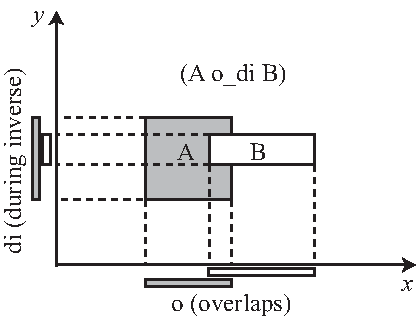
\includegraphics{block-algebra}}
\caption{\label{fig:block-algebra}Example relation o\_di in the block algebra}
\end{figure}

\clearpage
\section{Cardinal Direction Calculus}\label{sec:carddir}

\kasten{
\subsubsection*{Cardinal Direction Calculus overview}
\begin{calcfeatures}
\feature{calculus identifier}{cardir}
\feature{calculus parameters}{none}
\feature{arity}{binary}
\feature{entity type}{2D points}
\feature{description}{describes the orientation of two point regarding and absolute orientation}
\feature{base relations}{N, NE, E, SE, S, SW, W, NW, EQ}
\lastfeature{references}{\citet{frank-ACSM:91}, \citet{ligozat98_carddir}}
\end{calcfeatures}
}


\citet{frank-ACSM:91} introduced the cardinal direction calculus.%
\footnote{\citeauthor{frank-ACSM:91} introduced two different variants, called projection-based and cone-based. This calculus definition implements the projection-based variant.}
The euclidian plane $\mathcal{P}$ is partitioned into regions
with respect to a reference point $R$ and a global
\emph{west-east/south-north} reference frame.
Any point $P\in\mathcal{P}$ belongs to
one of the nine basic relations:
\textbf{N}orth, \textbf{N}orth\textbf{E}ast,
\textbf{E}ast, \textbf{S}outh\textbf{E}ast,
\textbf{S}outh, \textbf{S}outh\textbf{W}est,
\textbf{W}est, \textbf{N}orth\textbf{W}est,
or \textbf{Eq}ual.
The model is depicted in Figure \ref{fig:CardDir}.

\begin{figure}[htp]
	\centering
	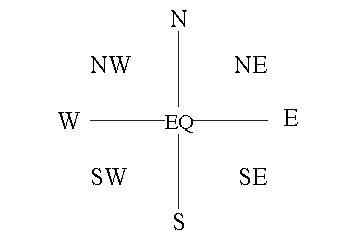
\includegraphics[width=0.5\textwidth]{CardDir_Projection}
	\caption{Base relations of the cardinal direction calculus.}
	\label{fig:CardDir}
\end{figure}



\clearpage
\section{The Region Connection Calculus family (RCC)}

The calculi from the RCC family (RCC-8 and RCC-5) allow
mereotopological reasoning (reasoning about connection and
part-of relationships) about simple regions in
the plane. Other domains involving regions
can also be considered in the context of RCC, e.g.\
3D regions, or non-simple regions in the plane,
which can affect the correctness of the
constraint-based reasoning algorithms.
Since so far no qualifier for RCC is available in \engine{},
the exact domain is actually still not determined. However, we
will assume the case of simple regions in the plane
in the following.


\subsection*{RCC-8}\label{sec:rcc8}

\kasten{
\subsubsection*{Region Connection Calculus 8 (RCC-8) overview}
\begin{calcfeatures}
\feature{calculus identifier}{rcc-8}
\feature{calculus parameters}{none}
\feature{arity}{binary}
\feature{entity type}{simple regions in the plane}
\feature{description}{describes the mereotopological relation between two regions}
\feature{base relations}{dc (disconnected), ec (externally connected),
po (partially overlapping), eq (equal), tpp (tangential proper part), ntpp (non-tangential proper part), tppi (tangential proper part inverse), ntppi (non-tangential proper part inverse)}
\feature{references}{\citet{randell92_rccb,Cohn97a}}
\lastfeature{remarks}{no qualifier is available for this calculus yet}
\end{calcfeatures}
}

RCC-8 is the more fine-grained variant of RCC calculi. It distinguishes
the eight base relations  dc (disconnected), ec (externally connected),
po (partially overlapping), eq (equal), tpp (tangential proper part), ntpp (non-tangential proper part), tppi (tangential proper part inverse), and nttpi (non-tangential proper part inverse) which are illustrated in Fig.~\ref{fig:RCC8}.

\begin{figure}[ht]
	\centering
	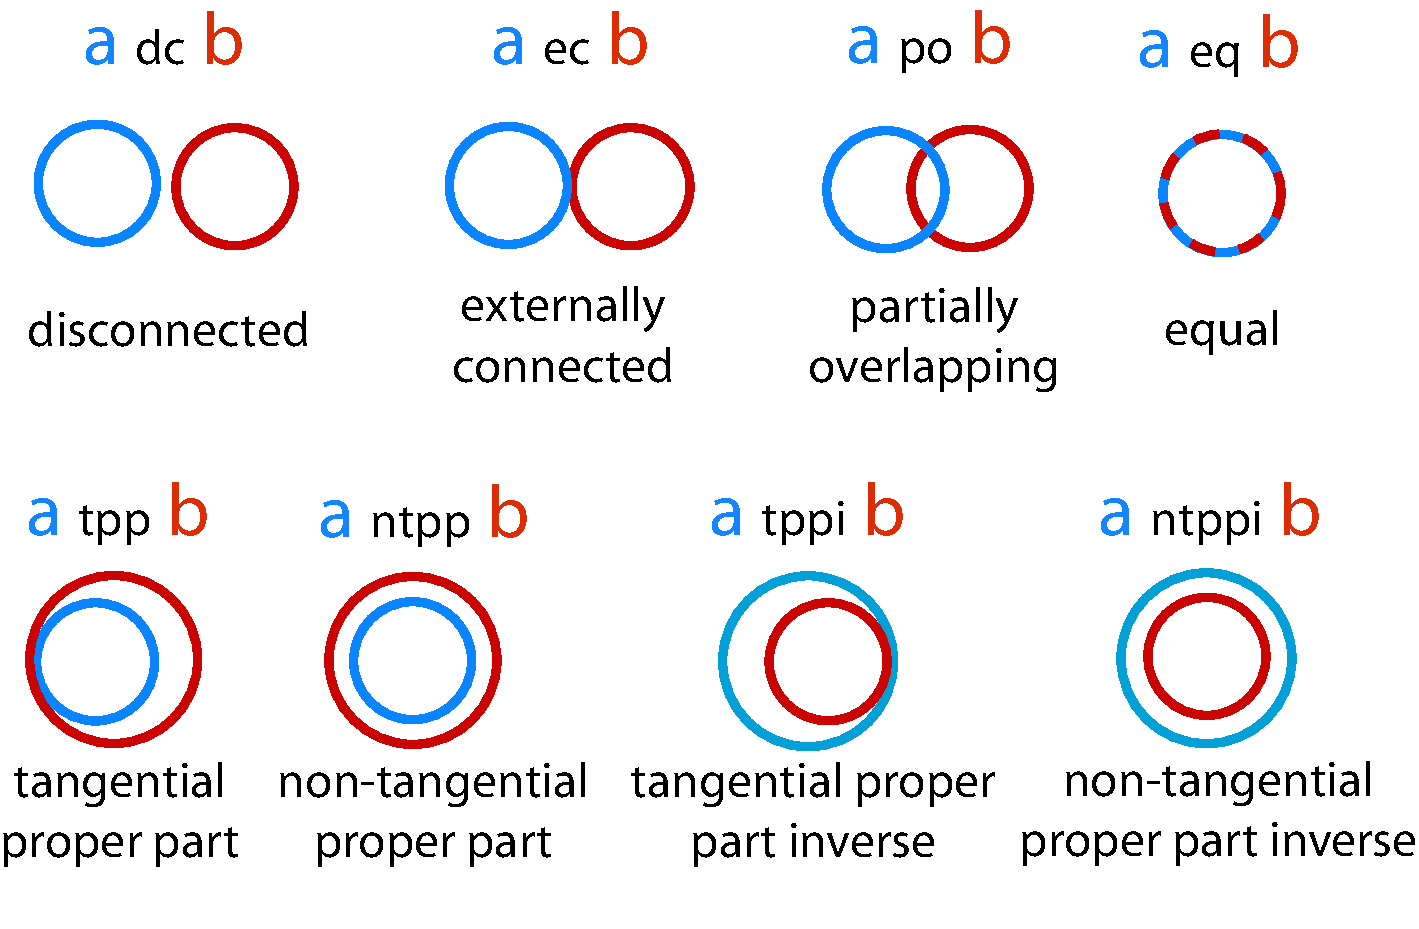
\includegraphics[width=0.70\textwidth]{RCC_new2}
	\caption{The RCC-8 base relations.}
	\label{fig:RCC8}
\end{figure}

\subsection*{RCC-5}\label{sec:rcc5}

\kasten{
\subsubsection*{Region Connection Calculus 5 (RCC-5) overview}
\begin{calcfeatures}
\feature{calculus identifier}{rcc-5}
\feature{calculus parameters}{none}
\feature{arity}{binary}
\feature{entity type}{simple regions in the plane}
\feature{description}{describes the mereotopological relation between two regions}
\feature{base relations}{dr (discrete from), po (partially overlapping), eq (equal),
pp (proper part), ppi (proper part inverse)}
\feature{references}{\citet{Cohn97a}}
\lastfeature{remarks}{no qualifier is available for this calculus yet}
\end{calcfeatures}
}

RCC-5 is a coarser version of RCC-8.  The RCC-8 relations
dc and ec are combined into one relation called dr. Similarly,
ntpp and tpp are combined into pp and ntppi and tppi into ppi.




\clearpage
\section{Dependency Calculus}\label{sec:depcalc}
%
\kasten{
\subsubsection*{Dependency Calculus overview}
\begin{calcfeatures}
\feature{calculus identifier}{depcalc, dep}
\feature{calculus parameters}{none}
\feature{arity}{binary}
\feature{entity type}{-}
\feature{description}{describes the order between nodes in a network}
\feature{base relations}{$<$, $=$, $>$, \^{}, $\sim$}
\feature{references}{\citet{Ragni05_DepCalc}, \citet{Ragni05_DepCalc_short}}
\lastfeature{remarks}{no qualifier is available for this calculus yet}
\end{calcfeatures}
}


The Dependency Calculus (DC) represents pairs of points regarding their
dependencies in a partial ordered structure.
Therefore, it meets all requirements to describe dependencies in networks.
If $x$, $y$ are points in a partial order $\langle T,\leq\rangle$
the base relations are defined as follows \citep{Ragni05_DepCalc}:
\begin{eqnarray*}
x < y & \text{iff} & x \leq y \text{ and not } y \leq x.\\
x = y & \text{iff} & x \leq y \text{ and } y \leq x.\\
x > y & \text{iff} & y \leq x \text{ and not } x \leq y.\\
x \text{ \^{} } y & \text{iff} & \exists z\; z \leq y \wedge z \leq x \text{ and neither } x \leq y \text{ nor } y \leq x.\\
x \sim y & \text{iff} & \text{ neither } \exists z\;z\leq y \wedge z \leq x \text{ nor } x\leq y \text{ nor } y\leq x .
\end{eqnarray*}



\clearpage

\section{Singlecross Calculus (SCC)}\label{sec:single-cross}

\kasten{
\subsubsection*{Singlecross calculus (SCC) overview}
\begin{calcfeatures}
\feature{calculus identifier}{scc}
\feature{calculus parameters}{none}
\feature{arity}{ternary}
\feature{entity type}{2D points}
\feature{description}{relates the referent c relative to the line between origin a and relatum b and the orthogonal line thru b, resulting in 11 base relations}
\feature{base relations}{0..7 and b (for b=c), dou, tri}
\lastfeature{references}{\citet{cosyfre92}}
\end{calcfeatures}
}

The single cross calculus is a ternary calculus that describes the direction of
a point $C$ (the referent) with respect to a point $B$ (the relatum) as seen
from a third point $A$ (the origin). It has originally been proposed in
\citet{cosyfre92}. The plane is partitioned into regions by the line going
through $A$ and $B$ and the perpendicular at $B$. This results in eight
possible directions for $C$ as illustrated in Fig.~\ref{fig:SCC}. We denote
these base relations by numbers from 0 to 7 instead of using linguistic
prepositions, e.g. 2 instead of \emph{left}, as originally done in
\citet{cosyfre92}. Relations 0, 2, 4, 6 are linear ones, while relations 1, 3,
5, 7 are planar. In addition, three special relations exist for the cases $A\neq
B=C$ (\textbf{b}), $A=B \neq C$ (\textbf{dou}), and $A=B=C$ (\textbf{tri}). A
single cross relation $rel_{SCC}$ is written as $A,B \; rel_{SCC}\; C$,
e.g. $A,B\; \textbf{4}\; C$ or $A,B\,\, \textbf{dou}\; C$. The relation depicted in Fig.~\ref{fig:SCC} is the relation $A,B\; \textbf{5}\; C$.

\begin{figure}[ht]
	\centering
	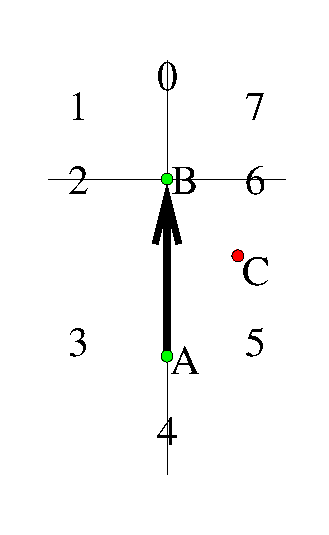
\includegraphics[height=4.3cm]{Singlecross}
	\caption{The Single Cross Reference System}
	\label{fig:SCC}
\end{figure}


\clearpage

\section{Doublecross Calculus (DCC)}\label{sec:double-cross}

\kasten{
\subsubsection*{Doublecross calculus (DCC) overview}
\begin{calcfeatures}
\feature{calculus identifier}{dcc, double-cross}
\feature{calculus parameters}{none}
\feature{arity}{ternary}
\feature{entity type}{2D points}
\feature{description}{relates the referent $C$ relative to the line between origin $A$ and relatum $B$ and the orthogonal lines through $A$ and $B$, resulting in 17 base relations}
\feature{base relations}{$0\uline 4$, $1\uline 5$, $2\uline 5$, $3\uline 5$, $3\uline 6$, $3\uline 7$, $4\uline 0$, $5\uline 1$, $5\uline 2$, $5\uline 3$, $6\uline 3$, $7\uline 3$, $4\uline 4$, $b\uline 4$, $4\uline a$, dou, tri}
\lastfeature{references}{\citet{cosyfre92}}
\end{calcfeatures}
}

The double cross calculus \citep{cosyfre92} can be seen as an extension of the single cross calculus adding another perpendicular, this time at $A$ (see Fig.~\ref{fig:DCC} (right)). It can also be interpreted as the combination of two single cross relations, the first describing the position of $C$ with respect to $B$ as seen from $A$ and the second with respect to $A$ as seen from $B$ (cf.~Fig.~\ref{fig:DCC} (left)). The resulting partition distinguishes 13 relations (7 linear and 6 planar) denoted by tuples derived from the two underlying SCC reference frames and four special cases, $A=C \neq B$ (\textbf{4\ul a}), $A\neq B=C$ (\textbf{b\ul 4}), $A=B \neq C$ (\textbf{dou}), and $A=B=C$ (\textbf{tri}), resulting in 17 base relations overall. In Fig.~\ref{fig:DCC} (right) the relation $A,B\; \textbf{5\ul 3}\; C$ is depicted.

\begin{figure}[ht]
	\centering
	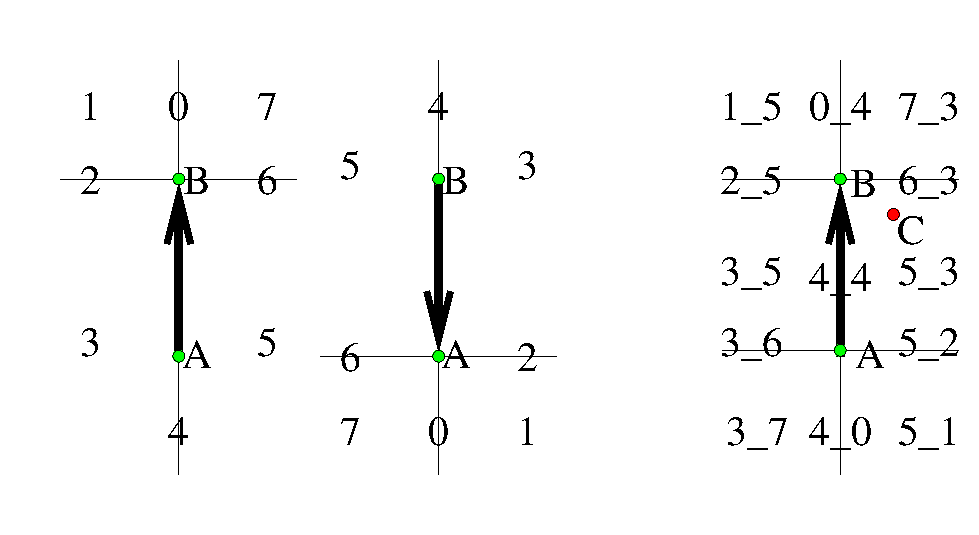
\includegraphics[height=4.3cm]{Doublecross_classic}
	\caption{The two Single Cross reference frames resulting in the overall Double Cross Calculus reference frame}
	\label{fig:DCC}
\end{figure}


\kasten{
\subsubsection*{Alternative Doublecross Calculus (DCC) overview}
\begin{calcfeatures}
\feature{calculus identifier}{adcc, alternative-double-cross}
\feature{calculus parameters}{none}
\feature{arity}{ternary}
\feature{entity type}{2D points}
\feature{description}{relates the referent $C$ relative to the line between origin $A$ and relatum $B$ and the orthogonal lines through $A$ and $B$, resulting in 17 base relations}
\feature{base relations}{0-12, a, b, dou, tri}
\lastfeature{references}{\citet{cosyfre92}}
\end{calcfeatures}
}

In the literature also a single numbered notation can be found.
We refer to this nomenclatur as the Alternative Doublecross Calculus.
Apart from relations $b\uline 4$, $4\uline a$ the mapping between tuple notation and alternative
notation is given in Figure \ref{fig:DCC_Table_alternative}.
$b\uline 4$ corresponds to \textbf{b} and $4\uline a$ to \textbf{a}.
\textbf{dou} and \textbf{tri} are defined as above.

\begin{figure}[h!]
	\centering
	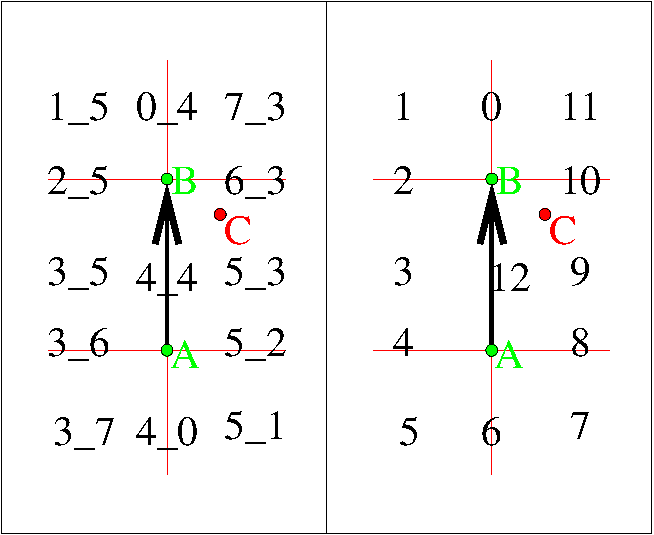
\includegraphics[height=4cm]{Doublecross_new}
	\caption{Schematic overview of Doublecross base relation names
	in tuple notation and the alternative notation.}
	\label{fig:DCC_Table_alternative}
\end{figure}



\clearpage
\section{FlipFlop Calculus With  $\mathcal{LR}$ Refinement} \label{sec:flip-flop}
% in case this will be added at some point
%
%
%

\kasten{
\subsubsection*{FlipFlop calculus (FFC) overview}
\begin{calcfeatures}
	\feature{calculus identifier}{ffc, ff, flipflop}
	\feature{calculus parameters}{none}
	\feature{arity}{ternary}
	\feature{entity type}{2D points}
	\feature{description}{relates the referent $C$ relative to the line segment starting at origin $A$ and ending at relatum $B$ resulting in nine base relations}
	\feature{base relations}{l (left), r (right), f (front), b (back), i (inside), s (start), e (end), dou, tri}
	\feature{references}{\citet{Ligozat93_FlipFlopCalculus,scivos:nebel:icsc-04}}
        \lastfeature{remark}{\engine{} uses the $\mathcal{LR}$ refinement in its implementation of the FFC}
\end{calcfeatures}
}

The FlipFlop calculus proposed in \citet{Ligozat93_FlipFlopCalculus}
describes the position of a
point $C$ (the referent) in the plane with respect to two other points
$A$ (the origin) and B (the relatum) as illustrated in Fig.
\ref{fig:FFC}. It can for instance be used to describe the spatial
relation of $C$ to $B$ as seen from $A$. For configurations with $A\neq B
$ the following base relations are distinguished: $C$ can be to the
\textbf{l}eft or to the \textbf{r}ight of the oriented line going
through $A$ and $B$, or $C$ can be placed on the line resulting in one of
the five relations \textbf{i}nside, \textbf{f}ront, \textbf{b}ack,
\textbf{s}tart ($C = A$) or \textbf{e}nd ($C = B$) (cp. Fig.
\ref{fig:FFC}). Relations for the case where $A$ and $B$ coincide were
not included in Ligozat's original definition
\citep{Ligozat93_FlipFlopCalculus}. This was done with the $\mathcal{LR}$
refinement \citep{scivos:nebel:icsc-04} that introduces the relations
\textbf{dou} ($A=B \neq C$) and \textbf{tri} ($A=B=C$) as additional
relations, resulting in 9 base relations overall. A $\mathcal{LR}$ relation $rel_\mathcal{LR}$
is written as $A,B\; rel_\mathcal{LR}\; C$, e.g. $A,B\; \textbf{r}\; C$ as depicted in Fig.~\ref{fig:FFC}.


\begin{figure}[htp]
	\centering
	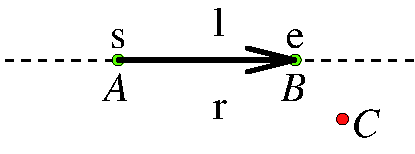
\includegraphics[width=0.4\textwidth]{flipflop_basenew}
	\caption{The reference frame for the $\mathcal{LR}$ calculus, an enhanced version
		 of the FlipFlop Calculus}
	\label{fig:FFC}
\end{figure}


\clearpage
\section{Cycord Family}\label{sec:cycord}

Cycord calculi \citep{isli98_2doriordering} are based on oriented line segments,
either defined by a direction directly, or start and end point (cf.~dipoles in \ref{sec:dipole}).
The relations between two line segments $X$ and $Y$ can take one of the four values:
 $e$ (equal alignment), 
 $l$ (oriented left, i.e.~the angle $\alpha$ between $X$ and $Y$ is $\alpha\in(0,\pi)$, 
 $o$ (opposite, i.e.~$\alpha=\pi$, or
 $r$ (oriented right, i.e.~$\alpha\in(\pi,2\pi)$.
The binary case, where two oriented line segments are related, is equivalent to the alignment calculus (Section \ref{sec:geomoricalc}).
In the ternary case three line segments are considered and the relation consists of a three tuple
$(r_{XY},r_{XZ},r_{YZ})$
with
$r_{XY}$ denoting the binary relation between $X$ and $Y$,
$r_{XZ}$ between $X$ and $Z$, and
$r_{YZ})$ between $Y$ and $Z$.
Out of the 64 possible only 24 are valid, i.e.~only 24 are consistent in terms of the binary Cycord definition.

\subsection*{Binary CyCord}\label{sec:cycord-binary}

\kasten{
\subsubsection*{Binary Cycord calculus overview}
\begin{calcfeatures}
\feature{calculus identifier}{cycord2, cc2}
\feature{calculus parameters}{none}
\feature{arity}{binary}
\feature{entity type}{dipoles in the plane (oriented line segments)}
\feature{description}{relates two dipoles regarding their relative orientation (alignment)}
\feature{base relations}{e, l, o, r}
\lastfeature{references}{\citet{isli98_2doriordering}, \cite{isli00_2doriordering}}
%\feature{remarks]
\end{calcfeatures}
}
\begin{figure}[ht]
 	\centering
	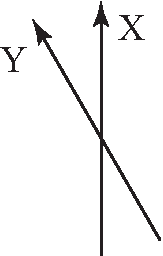
\includegraphics[width=0.15\textwidth]{cycord-binary}
	\caption{A binary Cycord relation: l}
	\label{fig:cc2}
\end{figure}

\subsection*{Ternary CyCord}\label{sec:cycord-binary}

\kasten{
\subsubsection*{Ternary Cycord calculus overview}
\begin{calcfeatures}
\feature{calculus identifier}{cycord3, cc3}
\feature{calculus parameters}{none}
\feature{arity}{ternary}
\feature{entity type}{dipoles in the plane (oriented line segments)}
\feature{description}{relates two dipoles regarding their relative orientation (alignment)}
\feature{base relations}{eee, ell, eoo, err, lel, lll, llo, llr, lor, lre, lrl, lrr, 
				     oeo, olr, ooe, orl, rer, rle, rll, rlr, rol, rrl, rro, rrr}
\lastfeature{references}{\citet{isli98_2doriordering}, \cite{isli00_2doriordering}}
%\feature{remarks]
\end{calcfeatures}
}
\begin{figure}[ht]
 	\centering
	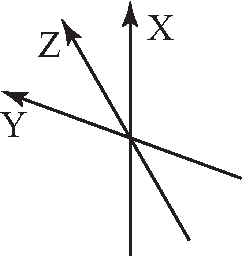
\includegraphics[width=0.15\textwidth]{cycord-ternary}
	\caption{A ternary Cycord relation: llr}
	\label{fig:cc3}
\end{figure}

\clearpage

\section{The Geometric Orientation (Alignment) Calculus}\label{sec:geomoricalc}

\kasten{
\subsubsection*{The Geometric Orientation (Alignment) Calculus overview}
\begin{calcfeatures}
\feature{calculus identifier}{geomori, ori, align}
\feature{calculus parameters}{none}
\feature{arity}{binary}
\feature{entity type}{dipole}
\feature{description}{describes the alignment of two oriented line segments}
% \feature{base relations}{\textbf{P}arallel, \textbf{+}, \textbf{-}, \textbf{O}pposite-parallel}
\feature{base relations}{$P$, $+$, $O$, $-$}
% \feature{references}{\citet{cosy:dylla:2004:qsnhinsitcalc_b}}
\feature{references}{\cite{cosy:dylla:2008:AgCtrlPerspOnQSR}, \cite{Dylla10_CombinedCalculus}}
\lastfeature{remarks}{no qualifier is available for this calculus yet;\\ conceptually equivalent to Binary Cycord (see Appendix \ref{sec:cycord-binary})}
\end{calcfeatures}
}

The Geometric Orientation Calculus, also called Geometric Alignment Calculus,
relates the alignment of two oriented line segments.
The alignment is derived by shifting both points of the second dipole
such that the starting points of dipole $A$ and $B$ coincide.
Dipole $B$ may point
in the same direction as $A$ (parallel),
in opposite direction as $A$ (opposite-parallel),
somewhere to the left of dipole $A$ (mathematically positive),
or somewhere to the right of dipole $A$ (mathematically negative).
An example with two dipoles which are aligned positively
is depicted in Figure \ref{fig:AlignCalc_Positive}.
The alignment of dipoles is part of the development of
the fine grained Dipole Relation Algebra with paralellism
in \citep{cosy:dylla:2004:qsnhinsitcalc_b}.


\begin{figure}[htb]
\begin{center}
%\addtolength{\abovedisplayshortskip}{-10pt}
%\addtolength{\abovedisplayskip}{-10pt}
\addtolength{\abovecaptionskip}{-15pt}
%\includegraphics[width=0.3\columnwidth]{pics/Dipole_Basic}
\scalebox{0.8}{\input{figures/DRAfp_rlll+_Example.pdf_t}}
\caption{Example of two dipoles which are aligned positively.}
\label{fig:AlignCalc_Positive}
\end{center}
\end{figure}



\clearpage
\section{Dipole Calculus Family}\label{sec:dipole}

A dipole is an oriented line segment as e.g.\ determined by a start and an end point. We will write $\vec{d}_{AB}$ for a dipole defined by start point $A$ and end point $B$.
The idea of using dipoles was first introduced by \citet{schlieder95_reasoning} and extended resulting in the coarse-grained Dipole Relation Algebra \DRAc{} \citep{moratz-renz-wolter-ECAI:00}. Later,
a fine-grained version of the dipole calculus ($\mathcal{DRA}_{f}$) has
been proposed \citep{cosy:dylla:2004:qsnhinsitcalc_b} and which has further been extended to $\mathcal{DRA}_{fp}$ \citep{cosy:dylla:2004:qsnhinsitcalc_b}.
In \engine{}, currently only the coarse-grained version \DRAc{} is available.


\subsection*{Coarse-grained Dipole Relation Algebra (\DRAc)}\label{sec:dipole-coarse}

\kasten{
\subsubsection*{Coarse-grained dipole calculus (\DRAc) overview}
\begin{calcfeatures}
\feature{calculus identifier}{dra-24, dipole-coarse}
\feature{calculus parameters}{none}
\feature{arity}{binary}
\feature{entity type}{dipoles in the plane (oriented line segments)}
\feature{description}{relates two dipoles using the FlipFlop relations
between the start and end point of one dipole and the other dipole}
\feature{base relations}{4-symbol words where each symbol can
be either l (left), r (right), s (start), or e (end) (not all combinations are possible)}
\lastfeature{references}{\citet{moratz-renz-wolter-ECAI:00}}
%\feature{remarks]
\end{calcfeatures}
}
\begin{figure}[ht]
 	\centering
% 	\includegraphics[width=0.4\textwidth]{DRAf_rlll+_Example}
	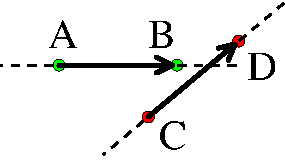
\includegraphics[width=0.3\textwidth]{dra-ex}
	\caption{A dipole configuration: $\vec{d}_{AB}~rlll~\vec{d}_{CD}$ in the coarse-grained dipole relation algebra ($\mathcal{DRA}_{c}$).}
	\label{fig:DRAf}
\end{figure}

The coarse-grained dipole calculus variant ($\mathcal{DRA}_{c}$) describes the orientation relation between two dipoles $\vec{d}_{AB}$ and  $\vec{d}_{CD}$ with the preliminary of $A$, $B$, $C$, and $D$ being in general position, i.e.\ no three disjoint points are collinear.
Each base relation is a 4-tuple $(r_1,r_2,r_3,r_4)$ of FlipFlop relations
relating a point from one of the dipoles with the other dipole.
$r_1$ describes the relation of $C$ with respect to the dipole  $\vec{d}_{AB}$, $r_2$ of $D$ with respect to  $\vec{d}_{AB}$, $r_3$ of $A$ with respect to $\vec{d}_{CD}$, and $r_4$ of $B$ with respect to $\vec{d}_{CD}$. The distinguished
FlipFlop relations are \textbf{l}eft, \textbf{r}ight, \textbf{s}tart,
and \textbf{e}nd (see Fig.~\ref{fig:FFC}). Dipole relations are usually written without commas and parentheses, e.g. $rrll$. Thus, the example in Fig.~\ref{fig:DRAf} shows the relation $\vec{d}_{AB}~rlll~\vec{d}_{CD}$.
Since the underlying points for a $\mathcal{DRA}_{c}$ relation need to be in
general position, $r_i$ can only take the values \textbf{l}eft, \textbf{r}ight, \textbf{s}tart, or \textbf{e}nd resulting in 24 base relations.


%\subsection*{fine grained dipole ($\mathcal{DRA}_{f}$)}
%
%A dipole is an oriented line segment as e.g. determined by a start and an end point. We will write $\vec{d}_{AB}$ for a dipole defined by start point $A$ and end point $B$. The fine-grained dipole calculus ($\mathcal{DRA}_{f}$) \ref{cosy:dylla:2004:qsnhinsitcalc_b} describes the orientation relation between two dipoles $\vec{d}_{AB}$ and  $\vec{d}_{CD}$. Each base relations is 4-tuple $(r_1,r_2,r_3,r_4)$ of FlipFlop relations. $r_1$ describes the relation of $C$ with respect to the dipole  $\vec{d}_{AB}$, $r_2$ of $D$ with respect to  $\vec{d}_{AB}$, $r_3$ of $A$ with respect to $\vec{d}_{CD}$, and $r_4$ of $b$ with respect to $\vec{d}_{CD}$. The relations are usually written without the commas, e.g. (rrll). Thus, the example in figure \ref{fig:DRAfp} s shows the relation $\vec{d}_{AB}$ (rlll) $\vec{d}_{CD}$. $\mathcal{DRA}_{f}$ has 72 base relations.
%
%\begin{figure}[htp]
%	\centering
%	\includegraphics[width=0.5\textwidth]{pics/DRAf_rlll+_Example}
%	\caption{A dipole configuration: $\vec{d}_{AB}$ (rlll) $\vec{d}_{CD}$ in the fine-grained dipole relation algebra ($\mathcal{DRA}_{f}$) or  $\vec{d}_{AB}$ (rlll+) $\vec{d}_{CD}$ in the extended version $\mathcal{DRA}_{fp}$.}
%	\label{fig:DRAfp}
%\end{figure}

% An extended version called $\mathcal{DRA}_{fp}$ \ref{cosy:dylla:2004:qsnhinsitcalc_b} further classifies the angle $s$  that would result from translating $\vec{d}_{CD}$ so that both start points coincide. Four cases are distinguished: \textbf{P}arallel ($s=0^\circ$), \textbf{A}ntiparallel ($s=180^\circ$), \textbf{+} ($s\in]0^\circ..180^\circ[$), and \textbf{-} ($s\in]180^\circ..360^\circ[$). This results in 80 base relations and the example from figure \ref{fig:DRAfp} depicts the  $\mathcal{DRA}_{fp}$ relation (rlll+).

%\subsection*{?}


\clearpage

\section{Oriented Point Reasoning Algebra With Granularity $m$ (\opra)}\label{sec:opra}

\kasten{
\subsubsection*{Oriented Point Relation Algebra (\opra) overview}
\begin{calcfeatures}
\feature{calculus identifier}{opra-}
\feature{calculus parameters}{granularity - number of partitioning lines (= number of planar relations / 2), must be $> 0$}
\feature{arity}{binary}
\feature{entity type}{oriented 2D points}
\feature{description}{relates two oriented points $a$ and $b$ with respect to granularity $m$}
\feature{base relations}{$[i,j]$ with $i, j$ $\in \{0,..,4m-1\}$, if $a$ and $b$ have different positions; $[i]$ with $i \in \{0,..,4m-1\}$ if they have the same position}
\lastfeature{references}{\citet{Moratz_Dylla_Frommberger_05_adjustable_Granularity,moratz06_opra}}
%\item[remarks]
\end{calcfeatures}
}

The domain of the Oriented Point Relation Algebra (\OPRAm{}) \citep{Moratz_Dylla_Frommberger_05_adjustable_Granularity,moratz06_opra} is the set of oriented points (points in the plane with an
additional direction parameter). The calculus relates two  oriented points
with respect to their relative orientation towards each other.
An oriented point
$\vec{O}$ can be described by its Cartesian coordinates $x_O, y_O \in {\mathbb{R}}$ and a direction $\phi_{\vec{O}} \in [0,2\pi]$ with respect to an absolute
reference direction and thus $D={\mathbb{R}}^2 \times [0,2\pi]$.

The \OPRAm{} calculus is suited for dealing with objects that have an intrinsic front or move in a particular direction and can be abstracted as points.
The exact set of base relations distinguished in  \OPRAm{} depends on the
granularity parameter $m\in \mathbb{N}$. For each of the two related oriented points, $m$ lines are used to partition the plane into $2m$ planar and $2m$ linear regions. Fig.~\ref{fig:OPRA} shows the partitions for the cases $m=2$
%(Fig.~\ref{fig:OPRA2})
(a) and $m=4$
%(\ref{fig:OPRA4})
(b). The orientation of the two points is depicted by the arrows starting at $\vec{A}$ and $\vec{B}$, respectively. The regions are numbered from 0 to $4m-1$; region 0 always coincides with the orientation of the point. An \OPRAm{} base relation $rel_{\mathcal{OPRA}_m}$ consists of a pair $(i,j)$ where
$i$ is the number of the region of $\vec{A}$ which contains $\vec{B}$, while $j$ is the number of the region of $\vec{B}$ that contains $\vec{A}$. These relations are usually written as $\vec{A} \; {\scriptscriptstyle m}\angle_{i}^{j} \; \vec{B}$ with $i,j\in \mathcal{Z}_{4m}$\footnote{$\mathcal{Z}_{4m}$ defines a cyclic group with $4m$ elements.}. Thus, the examples in Fig.~\ref{fig:OPRA} depict the relations $\vec{A} \; {\scriptscriptstyle 2}\angle_{7}^{1} \; \vec{B}$ and $\vec{A} \; {\scriptscriptstyle 4}\angle_{13}^{3} \; \vec{B}$. Additional base relations called \emph{same relations} describe situations in which the positions of both oriented points coincide. In these cases, the relation is determined by the number $s$ of the region of $\vec{A}$
into which the orientation arrow of $\vec{B}$ falls (as illustrated in Fig.~\ref{fig:OPRA2same}). These relations are written as $\vec{A} \; {\scriptscriptstyle 2}\angle s \; \vec{B}$ ($\vec{A} \; {\scriptscriptstyle 2}\angle 1 \; \vec{B}$ in the example).

The complete set $\mathcal{R}$ of \OPRAm{} relations is the power set
of the base relations described above.
% \marginpar{FD: $2^{[(4m)^2+4m]}$ sagen?}

\begin{figure}[tb!]
% \begin{center}
\begin{flushleft}
	\subfigure[$m=2$: $\vec{A} \; {\scriptscriptstyle 2}\angle_{7}^{1} \; \vec{B}$]{
% 	\subfigure[with $m=2$: $\vec{A} \; {\scriptscriptstyle 2}\angle_{7}^{1} \; \vec{B}$]{
		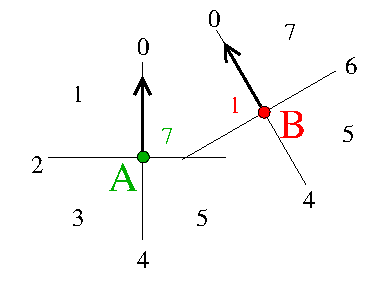
\includegraphics[width=0.307\textwidth]{OPRA2_Example}
		\label{fig:OPRA2}
	}
	\subfigure[$m=4$: $\vec{A} \; {\scriptscriptstyle 4}\angle_{13}^{3} \; \vec{B}$]{
% 	\subfigure[with $m=4$: $\vec{A} \; {\scriptscriptstyle 4}\angle_{13}^{3} \; \vec{B}$]{
		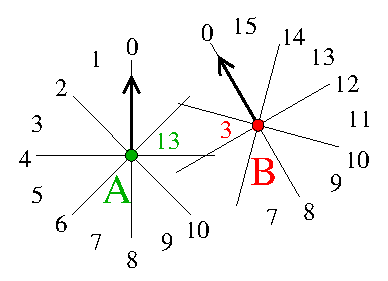
\includegraphics[width=0.307\textwidth]{OPRA4_Example}
		\label{fig:OPRA4}
	}
	\subfigure[case where $\vec{A}$ and $\vec{B}$ coincide: $\vec{A} \; {\scriptscriptstyle 2}\angle 1 \; \vec{B}$]{
		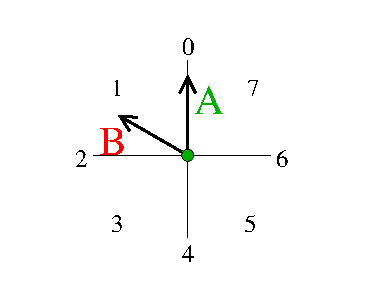
\includegraphics[width=0.307\textwidth]{OPRA2_ExampleSame}
		\label{fig:OPRA2same}
	}
	\caption{Two oriented points related at different granularities.}
	\label{fig:OPRA}
\end{flushleft}
% \end{center}
\end{figure}


\clearpage
\section{Point Calculus (Point Algebra)}\label{sec:pointcalc}

\kasten{
\subsubsection*{Point Calculus (Point Algebra) overview}
\begin{calcfeatures}
\feature{calculus identifier}{point-calculus, pc, point-algebra, pa}
\feature{calculus parameters}{none}
\feature{arity}{binary}
\feature{entity type}{1D points}
\feature{description}{describes the order between two 1D points (values)}
\feature{base relations}{$<$, $=$, $>$}
\lastfeature{references}{\citet{vilain_kautz_beek_89_constraint}}
\end{calcfeatures}
}

The Point Calculus (PC) \citep{vilain_kautz_beek_89_constraint} relates pairs of
1D points, represented by real-valued numbers. Pairs of values are categorized using the three base relations less than ($<$), equal ($=$), or greater than ($>$).



\clearpage

\section{Qualitative Trajectory Calculus Family}\label{sec:qtc}
\citet{Weghe04_PhD} developed a family of trajectory calculi on the basis of relative trajectories of two moving objects.
He investigates representation where he combined subsets of the three different features:
change in distance, change to the side, and relative velocity.
He also investigated differences in representations based on one dimensional (1D) and two dimensional (2D) entities.
The most basic calculus is $QTC_{B11}$ dealing with change in distance in 1D,
enhanced with velocity in $QTC_{B12}$.
The extensions to 2D entities is given in $QTC_{B21}$ and $QTC_{B22}$.
$QTC_{C21}$ ($QTC_{C22}$) extends $QTC_{B21}$ ($QTC_{B22})$ by relative velocity.


\subsection*{QTC in 1D With Distance}\label{sec:qtc-b11}
\kasten{
\subsubsection*{Qualitative Trajectory Calculus in 1D (QTC-B11)}
\begin{calcfeatures}
\feature{calculus identifier}{qtc-b11}
\feature{calculus parameters}{none}
\feature{arity}{binary}
\feature{entity type}{interval (1D trajectory positions at two different time points)}
\feature{description}{describes the relative orientation between two trajectory segments}
\feature{base relations\footnotemark}{++, +-, +O, -+, - -, -O, O+, O-, OO}
\feature{references}{\citet{Weghe04_PhD}}
\lastfeature{remarks}{no qualifier is available for this calculus yet}
\end{calcfeatures}
}
\footnotetext{For avoiding the necessity to quote every single relation
such that leading zeros are not ignored we realized the implementation with O's
instead of zeros.}

$QTC_{B11}$ represents the relative distance change of two moving objects $A$ and $B$ at
timepoints $t_i$ and $t_{i+1}$ .
Intuitively, the first character denotes whether $A$ moves towards the starting position of $B$ ($-$), moves away ($+$, or the distance stays the same ($O$).
With $dist(x,y)$ denoting the distance between two positions
and $A_i$ denotes the position of object $A$ at time point $t_i$
moving towards means $dist(A_{i+1}, B_{i})<dist(A_{i}, B_{i})$,
moving away means $dist(A_{i+1}, B_{i})>dist(A_{i}, B_{i})$,
and equidistant means $dist(A_{i+1}, B_{i})=dist(A_{i}, B_{i})$
The second character represents the change in distance regarding $B$ wrt. $A$.
This results in nine base relations.


\subsection*{QTC in 1D With Distance and Velocity}\label{sec:qtc-b12}
\kasten{
\subsubsection*{Qualitative Trajectory Calculus in 1D with velocity (QTC-B12)}
\begin{calcfeatures}
\feature{calculus identifier}{qtc-b12}
\feature{calculus parameters}{none}
\feature{arity}{binary}
\feature{entity type}{-}
\feature{description}{describes the relative orientation between two trajectory segments}
\feature{base relations}{+++, ++-, ++O, +-+, +- -, +-O, +O+, -++, -+-, -+O, - -+, - - -, - -O, -O+, O+-, O- -, OOO}
\feature{references}{\citet{Weghe04_PhD}}
\lastfeature{remarks}{no qualifier is available for this calculus yet}
\end{calcfeatures}
}

The first two characters of $QTC_{B12}$ represent the same as $QTC_{B11}$.
The third character represents the relative velocitiy between $A$ and $B$,
i.e.~whether object $A$ is slower than $B$ ($-$), is faster ($+$), or both have the same velocity ($O$). Because the conditions of the three characters interfere in 1D
only 17 out of 27 potential relations are feasible.


\subsection*{QTC in 2D With Distance}\label{sec:qtc-b21}
\kasten{
\subsubsection*{Qualitative Trajectory Calculus in 2D (QTC-B21)}
\begin{calcfeatures}
\feature{calculus identifier}{qtc-b21}
\feature{calculus parameters}{none}
\feature{arity}{binary}
\feature{entity type}{dipole (2D trajectory positions at two different time points)}
\feature{description}{describes the relative orientation between two trajectory segments}
\feature{base relations}{++, +-, +O, -+, - -, -O, O+, O-, OO}
\feature{references}{\citet{Weghe04_PhD}}
\lastfeature{remarks}{no qualifier is available for this calculus yet}
\end{calcfeatures}
}

$QTC_{B21}$ is similar to $QTC_{B11}$ except dealing with trajectories in 2D instead of only 1D.


\subsection*{QTC in 2D With Distance and Velocity}\label{sec:qtc-b22}
\kasten{
\subsubsection*{Qualitative Trajectory Calculus in 2D with velocity (QTC-B22)}
\begin{calcfeatures}
\feature{calculus identifier}{qtc-b22}
\feature{calculus parameters}{none}
\feature{arity}{binary}
\feature{entity type}{-}
\feature{description}{describes the relative orientation between two trajectory segments}
\feature{base relations}{ $\{+,O,-\}\times\{+,O,-\}\times\{+,O,-\}$}
\feature{references}{\citet{Weghe04_PhD}}
\lastfeature{remarks}{no qualifier is available for this calculus yet}
\end{calcfeatures}
}

$QTC_{B22}$ is similar to $QTC_{B12}$ except dealing with trajectories in 2D instead of only 1D.
In contrast to $QTC_{B12}$ in 2D all 27 potential relations are feasible.



\subsection*{QTC in 2D With Distance and Side}\label{sec:qtc-c21}
\kasten{
\subsubsection*{Qualitative Trajectory Calculus in 2D (QTC-C21)}
\begin{calcfeatures}
\feature{calculus identifier}{qtc-c21}
\feature{calculus parameters}{none}
\feature{arity}{binary}
\feature{entity type}{dipole (2D trajectory positions at two different time points)}
\feature{description}{describes the relative orientation between two trajectory segments}
\feature{base relations}{$\{+,O,-\}\times\{+,O,-\}\times\{+,O,-\}\times\{+,O,-\}$}
\feature{references}{\citet{Weghe04_PhD}}
\lastfeature{remarks}{no qualifier is available for this calculus yet}
\end{calcfeatures}
}

$QTC_{C21}$ relations are given by a four character tuple.
The first two characters represent the same as a $QTC_{B21}$ relation.
The third character denotes whether $A$ moves to the left ($-$), to the right ($+$),
or on the reference line ($O$) spanned between $A$ and $B$ at $t_i$.
The fourth character represents the change of $B$ wrt. to this reference line.
This results in $3^4=81$ base relations.


\subsection*{QTC in 2D With Distance, Side, and Velocity}\label{sec:qtc-c22}
\kasten{
\subsubsection*{Qualitative Trajectory Calculus in 2D with velocity (QTC-C22)}
\begin{calcfeatures}
\feature{calculus identifier}{qtc-c22}
\feature{calculus parameters}{none}
\feature{arity}{binary}
\feature{entity type}{-}
\feature{description}{describes the relative orientation between two trajectory segments}
\feature{base relations}{$\{+,O,-\}\times\{+,O,-\}\times\{+,O,-\}\times\{+,O,-\}\times\{+,O,-\}$}
\feature{references}{\citet{Weghe04_PhD}}
\lastfeature{remarks}{no qualifier is available for this calculus yet}
\end{calcfeatures}
}

$QTC_{C22}$ relations are given by a five character tuple.
The first four directly map onto $QTC_{C21}$ relations.
The fifth character represents the relative velocity between objects $A$ and $B$.
$-$ denotes $A$ being slower than $B$ , $+$ is faster, and $O$ if both move at the same speed.






%\section{Ternary Point Configuration calculus (TPCC)}

%\kasten{
%\subsubsection*{Ternary Point Configuration Calculus (TPCC) overview}
%\begin{description}
%\item[short name] tpcc
%\item[calculus parameters] none
%\item[arity] ternary
%\item[entity type] 2D points
%\item[description] relates three points (origin, relatum, and referent) with respect to the relative distance between origin and relatum (derived from the double cross calculus)
%\item[base relations] sam, dou, tri, csb, dsb, clb, dlb, cbl, dbl, csl, dsl, cfl, dfl, clf, dlf, csf, dsf, crf, drf, cfr, dfr, csr, dsr, cbr, dbr, crb, drb
%\item[references]  \citet{moratz03_qsr_relpos}
%\end{description}
%}

%\chapter{Technical Details}
%\label{sec:technical-details}

\chapter{Quick Reference}

\section{Command Summary}
\section*{\tt compute-relation c op arg-1 \{arg-i\}}

Applies operation {\tt op} of calculus {\tt c} to arguments. Operations:
\begin{longtable}{|l|p{10cm}|}
\hline
\multicolumn{2}{|l|}{\bf spatial:}\\ \hline
{\tt composition, comp} & $ r s \mapsto r \circ s$\\
{\tt converse, cnv}\binaryonly & $r \mapsto r^{\smile}$ \\
{\tt homing, hm}\ternaryonly & $ r \mapsto hm(r)$\\
{\tt homingi, hmi}\ternaryonly & $ r \mapsto inv(hm(r))$\\
{\tt inverse, inv}\ternaryonly & $ r \mapsto inv(r)$\\
{\tt shortcut, sc}\ternaryonly & $ r \mapsto sc(r)$\\
{\tt shortcuti, sci}\ternaryonly & $ r \mapsto inv(sc(r))$\\[1ex]
\hline
\multicolumn{2}{|l|}{\raisebox{-2ex}[2ex][2.5ex]{{\bf calculi-theoretic:}}}\\ \hline
{\tt closure} & $ r_1 r_2 \ldots r_n \mapsto Cl(r_1,r_2,\ldots, r_n)$\newline
$Cl$ denotes the minimal set of relations that is closed under composition, converse,
and intersection\\
{\tt base-closure} & $Cl(br_1,br_2,\ldots , br_n)$\newline
Computes closure of the set of base relations\\
\hline
\multicolumn{2}{|l|}{\raisebox{-2ex}[2ex][2.5ex]{{\bf set-theoretic:}}}\\ \hline
{\tt complement, cmpl} & $ r \mapsto r^C$\\
{\tt minus} & $ r s \mapsto r \backslash s$\\
{\tt union} & $ r s \mapsto r \cup s$\\
{\tt intersection, isec} & $ r s \mapsto r \cap s$\\
\hline
\end{longtable}
For complex operations a Lisp-style prefix syntax can be used, i.e., nested expression enclosed by parantheses, e.g., {\tt (composition rel1 (inverse (homing rel2)))} computes rel1$\circ$ inv(hom(rel2))

\section*{\tt analyze-calculus c op}
Determines relation-algebraic properties
\begin{description}
	\item[{\tt c}] calculus
	\item[{\tt op}] operation:
	\begin{longtable}{|lp{6cm}|}
	\hline
{\tt analyze-calculus c test-algebra} &  checks which axioms are met by the algebraic structure of the calculus\\
{\tt analyze-calculus c test-property prop} &  checks whether axiom {\tt prop} is satisfied by the calculus\\
\hline
\end{longtable}
\end{description}

\section*{\tt qualify c opt scene}
Determines qualitative configuration from quantitative scene description.
	\begin{description}
		\item[{\tt c}] calculus
		\item[{\tt opt}] either {\tt first2all} or {\tt all}, sets which objects to relate
		\item[{\tt scene}] list of lists containing objects id and coordinates, e.g. {\tt ((Point-A 12.2 34.8) (Point-B -2.3 28.8))}
	\end{description}

\section*{\tt constraint-reasoning c op conf1 [conf2]}

Performs operation {\tt op} on qualitative configuration with respect to calculus {\tt c}:
\begin{longtable}{|p{4.5cm}|p{9cm}|}
\hline
\multicolumn{2}{|l|}{\bf consistency checking:}\\ \hline
{\tt algebraic-closure}, {\tt a-closure}, {\tt path-consistency}  & Enforces path-consistency --- since this is a purely syntactical operation on the
					level of qualitative relations the term ``algebraic closure'' is more adequate.
					However, since ``path-consistency'' is widely used in this meaning, this name is
					supported too.\\
{\tt scenario-consistency} & Computes consistent networks containing base-relations only\\[0,5ex]
{\tt ternary-closure} & Computes algebraically closed networks using ternary composition with ternary calculi\\[1,0ex]
\hline
\multicolumn{2}{|l|}{\raisebox{-2ex}[2ex][2.5ex]{{\bf manipulating constraint networks:}}}\\ \hline
{\tt refine} & Merges two networks by intersecting corresponding constraints\\
{\tt extend} & Merges two networks by uniting corresponding constraints\\
{\tt update} & Merges two networks by overwriting corresponding constraints\\ \hline
\end{longtable}

\section*{\tt a-reasoning c cmd args}
Algebraic reasoning commands (see Sec.~\ref{sec:a-reasoning} starting on page \pageref{sec:a-reasoning}), {\tt c} designates calculus to use, command {\tt cmd} and arguments are {\tt args}:

\begin{longtable}{|l|l|p{68mm}|}
\hline
{\bf command} & {\bf arguments} & {\bf decription}\\ \hline
{\tt consistency} & constraint-nework & tests network for satisfiability, answers:
\begin{description}
	\item[{\tt SATISFIABLE.}] network proven to be consistent
	\item[{\tt NOT SATISFIABLE.}] network proven to be inconsistent
	\item[{\tt CANNOT DECIDE.}] neither of the above
\end{description}
\\
{\tt analyze-operation} & operation & Verifies operation table; operation is e.g., {\tt composition}, {\tt converse}, {\tt inverse}, {\tt shortcut}, $\ldots$\\
{\tt qualify} & scene opt & qualification, arguments as for the qualify model (see above) but based purely on the algebraic specification\\ \hline
\end{longtable}

\section*{\tt export c format}

Exports calculus definition of {\tt c} in {\tt format}:
\begin{description}
	\item[{\tt qat}] XML specification for QAT toolkit
	\item[{\tt gqr}] specification for GQR constraint reasoner
\end{description}


\section{Interactive Mode}

Using \engine in the interactive mode (i.e., invoking it with the ``-i'' command line option) some additional commands are available:
\pagebreak[4]

\begin{longtable}{|lp{10cm}|}\hline
	{\bf command} & {\bf description} \\ \hline \hline
	{\tt quit} & exits \engine{}\\
	{\tt help} & prints short help message\\
	{\tt load-calculus CALC} & loads a specified calculus into memory\\
	{\tt *} & used as calculus specifier in commands, {\tt *} stands for the calculus recently loaded into memory. This avoids overhead of reloading a calculus\\ \hline
\end{longtable}

\section{List of Calculi}
\renewcommand{\arraystretch}{1.5}
\begin{center}
\begin{longtable}{|p{4cm}p{6cm}ll|}\hline
	{\bf calculus identifier(s)} & {\bf calculus} & {\bf section} & {\bf page}\\ \hline \hline
%
	{\tt allen, aia, ia} & Allen's interval algebra \citep{allen83} & \ref{sec:allen} & \pageref{sec:allen} \\
	{\tt block-algebra, ba} & 2D block algebra \citep{guesgen:89} & \ref{sec:block-algebra} & \pageref{sec:block-algebra}\\
	{\tt cardir} & Cardinal direction calculus \citep{ligozat98_carddir}  & \ref{sec:carddir} & \pageref{sec:carddir} \\
	{\tt depcalc, dep} & Dependency calculus \citep{Ragni05_DepCalc} & \ref{sec:depcalc} & \pageref{sec:depcalc} \\
	{\tt dipole-coarse, dra-24} & Dipole calculus \citep{moratz-renz-wolter-ECAI:00} & \ref{sec:dipole-coarse} & \pageref{sec:dipole-coarse} \\
	{\tt double-cross, dcc} & Double cross calculus \citep{cosyfre92} using the original tuple naming scheme & \ref{sec:double-cross} & \pageref{sec:double-cross} \\
	{\tt alternative-double- cross, adcc} & Double cross calculus \citep{cosyfre92} using the alternative single number naming scheme & \ref{sec:double-cross} & \pageref{sec:double-cross} \\
	{\tt flipflop, ffc, ff} & FlipFlop calculus \citep{Ligozat93_FlipFlopCalculus}& \ref{sec:flip-flop} & \pageref{sec:flip-flop} \\
	{\tt geomori, ori, align} & Geometric Orientation calculus & \ref{sec:geomoricalc} & \pageref{sec:geomoricalc} \\
	{\tt point-calculus, pc, point-algebra, pa} & Point algebra \citep{vilain_kautz_beek_89_constraint} & \ref{sec:pointcalc} & \pageref{sec:pointcalc} \\
	{\tt rcc-5} & Region connection calculus (RCC-5) \citep{randell92_rccb} & \ref{sec:rcc5} & \pageref{sec:rcc5} \\
	{\tt rcc-8} & Region connection calculus (RCC-8) \citep{randell92_rccb} & \ref{sec:rcc8} & \pageref{sec:rcc8} \\
	{\tt reldistcalculus} & Exemplary calculus from this manual & \ref{sec:calculus-spec} & \pageref{sec:calculus-spec}\\
	{\tt single-cross, scc} & Single cross calculus \citep{cosyfre92} & \ref{sec:single-cross} & \pageref{sec:single-cross} \\
	{\tt opra-} & Oriented point reasoning algebra (\opra{})\citep{moratz06_opra} & \ref{sec:opra} & \pageref{sec:opra}\\
	{\tt qtc-b11} & Qualitative trajectory calculus in 1D with distance \citep{Weghe04_PhD} & \ref{sec:qtc-b11} & \pageref{sec:qtc-b11}\\
	{\tt qtc-b12} & Qualitative trajectory calculus in 1D with velocity \citep{Weghe04_PhD} & \ref{sec:qtc-b12} & \pageref{sec:qtc-b12}\\
	{\tt qtc-b21} & Qualitative trajectory calculus in 2D with distance \citep{Weghe04_PhD} & \ref{sec:qtc-b21} & \pageref{sec:qtc-b21}\\
	{\tt qtc-b22} & Qualitative trajectory calculus in 2D with distance and velocity \citep{Weghe04_PhD} & \ref{sec:qtc-b22} & \pageref{sec:qtc-b22}\\
	{\tt qtc-c21} & Qualitative trajectory calculus in 2D with distance and side \citep{Weghe04_PhD} & \ref{sec:qtc-c21} & \pageref{sec:qtc-c21}\\
	{\tt qtc-c22} & Qualitative trajectory calculus in 2D with distance, side, and velocity \citep{Weghe04_PhD} & \ref{sec:qtc-c22} & \pageref{sec:qtc-c22}\\
	\hline
\end{longtable}
\end{center}
\renewcommand{\arraystretch}{1.0}

\end{document}
